\documentclass[9pt]{beamer}

\usepackage[T1]{fontenc}
\usepackage[utf8]{inputenc}

\usepackage{graphicx}
\usepackage[export]{adjustbox}  % graphics alignment
\usepackage{helvet}  % helvetica
\usepackage[symbolgreek]{mathastext}  % equations in the same font as text
\usepackage{amsmath}
\usepackage{textcomp}
\usepackage{color,colortbl}
\usepackage{tikz}  % vector graphics
\usetikzlibrary{shapes,arrows,positioning}
\usepackage{ulem}  % underlining, striking text
\usepackage[font=normalsize,labelformat=simple]{subfig} 
\usepackage{xcolor}  % color text
\usepackage{hyperref}
\usepackage{siunitx}  % SI units
\sisetup{output-decimal-marker={,}}

\newcounter{saveenumi}
\newcommand{\seti}{\setcounter{saveenumi}{\value{enumi}}}
\newcommand{\conti}{\setcounter{enumi}{\value{saveenumi}}}

\resetcounteronoverlays{saveenumi}

\renewcommand{\thesubfigure}{\relax}  % Do nothing for the counter »subfigure«

\setbeamerfont{footnote}{size=\tiny}
\setbeamercovered{transparent}

\usetheme[
%%% options passed to the outer theme
%    hidetitle,           % hide the (short) title in the sidebar
%    hideauthor,          % hide the (short) author in the sidebar
%    hideinstitute,       % hide the (short) institute in the bottom of the sidebar
%    shownavsym,          % show the navigation symbols
%    width=2cm,           % width of the sidebar (default is 2 cm)
%    hideothersubsections,% hide all subsections but the subsections in the current section
%    hideallsubsections,  % hide all subsections
%    left                % right of left position of sidebar (default is right)
]{Aalborg}

%%% Macro para colorir linha da tabela
\makeatletter
  \def\rowcolor{\noalign{\ifnum0=`}\fi\bmr@rowcolor}
  \newcommand<>{\bmr@rowcolor}{%
    \alt#1%
    {\global\let\CT@do@color\CT@@do@color\@ifnextchar[\CT@rowa\CT@rowb}% 
    {\ifnum0=`{\fi}\@gooble@rowcolor}% 
  }
  \newcommand{\@gooble@rowcolor}[2][]{\@gooble@rowcolor@}
  \newcommand{\@gooble@rowcolor@}[1][]{\@gooble@rowcolor@@}
  \newcommand{\@gooble@rowcolor@@}[1][]{\ignorespaces}
\makeatother
%%% Macro termina aqui

\title[T\&P de Ferros Fundidos Nodulares]{Têmpera e Partição de Ferros Fundidos Nodulares: Microestrutura e Cinética}
\author[Arthur Nishikawa]{\emph{Arthur Seiji Nishikawa}\\Orientador: Prof. Hélio Goldenstein\\Coorientador: Prof. André Paulo Tschiptschin}
\institute[Depto. de Engenharia Metalúrgica e de Materiais - EPUSP]{Departamento de Engenharia Metalúrgica e de Materiais\\
      Escola Politécnica - Universidade de São Paulo}
\date{1º de outubro de 2018}

\pgfdeclareimage[width=1cm]{mainlogo}{AAUgraphics/EP-Circular.pdf}
\logo{\pgfuseimage{mainlogo}}

\AtBeginSection[]{
  \begin{frame}<beamer>{Sumário}
    \tableofcontents[currentsection]
  \end{frame}
}

\pgfdeclareimage[width=2cm]{titlepagelogo}{AAUgraphics/EP-Circular.pdf}
\titlegraphic{
  \pgfuseimage{titlepagelogo}
}

\begin{document}

% \begin{frame}
%   \begin{figure}
%   \href{img/test.mp4}{
%     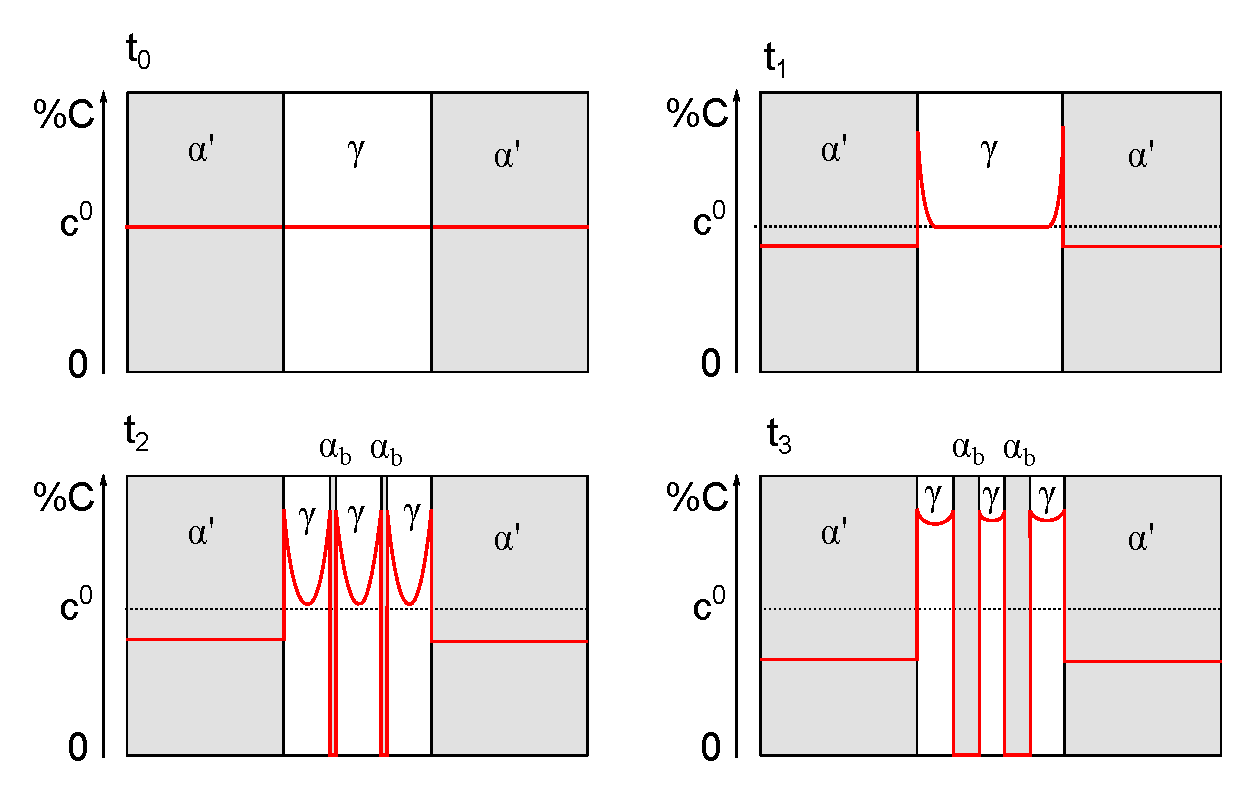
\includegraphics[width=.8\textwidth]{img/C_profiles.pdf}
%   }
%   \end{figure}
% \end{frame}
\begin{frame}[plain,noframenumbering]
  \titlepage
\end{frame}

\begin{frame}{Sumário}
  \tableofcontents
\end{frame}

\section{Introdução e objetivos}

\begin{frame}{Introdução}
  \begin{itemize}
    \item O processo de \textbf{Têmpera e Partição}\footnotemark[1] (T\&P) foi inicialmente proposto como rota de tratamento térmico para obtenção de \textbf{microestruturas multifásicas} compostas de martensita e substanciais quantidades de \textbf{austenita enriquecida em carbono}
    \item A \textbf{martensita} ($\alpha'$) confere \textbf{alta resistência}, enquanto \textbf{austenita} ($\gamma$) favorece \textbf{ductilidade} pela ocorrência do fenômeno de transformação martensítica induzida por deformação (TRIP)
  \end{itemize}

  \footnotetext[1]{Speer J, Matlock DK, De Cooman BC, Schroth JG. Acta Mater 2003;51:2611.}
\end{frame}

\begin{frame}{Introdução}
  \begin{itemize}
    \item Têmpera parcial a $Mf < T_T < Ms$ para formar quantidade controlada de $\alpha'$
    \item Reaquecido até $T_P$ para redistribuir C de $\alpha'$ para $\gamma$ (partição)
    \item C diminui Ms de $\gamma$, estabilizando-a a temperatura ambiente
    \item Si e Al adicionados para atrasar precipitação de cementita
  \end{itemize}

  \begin{figure}
    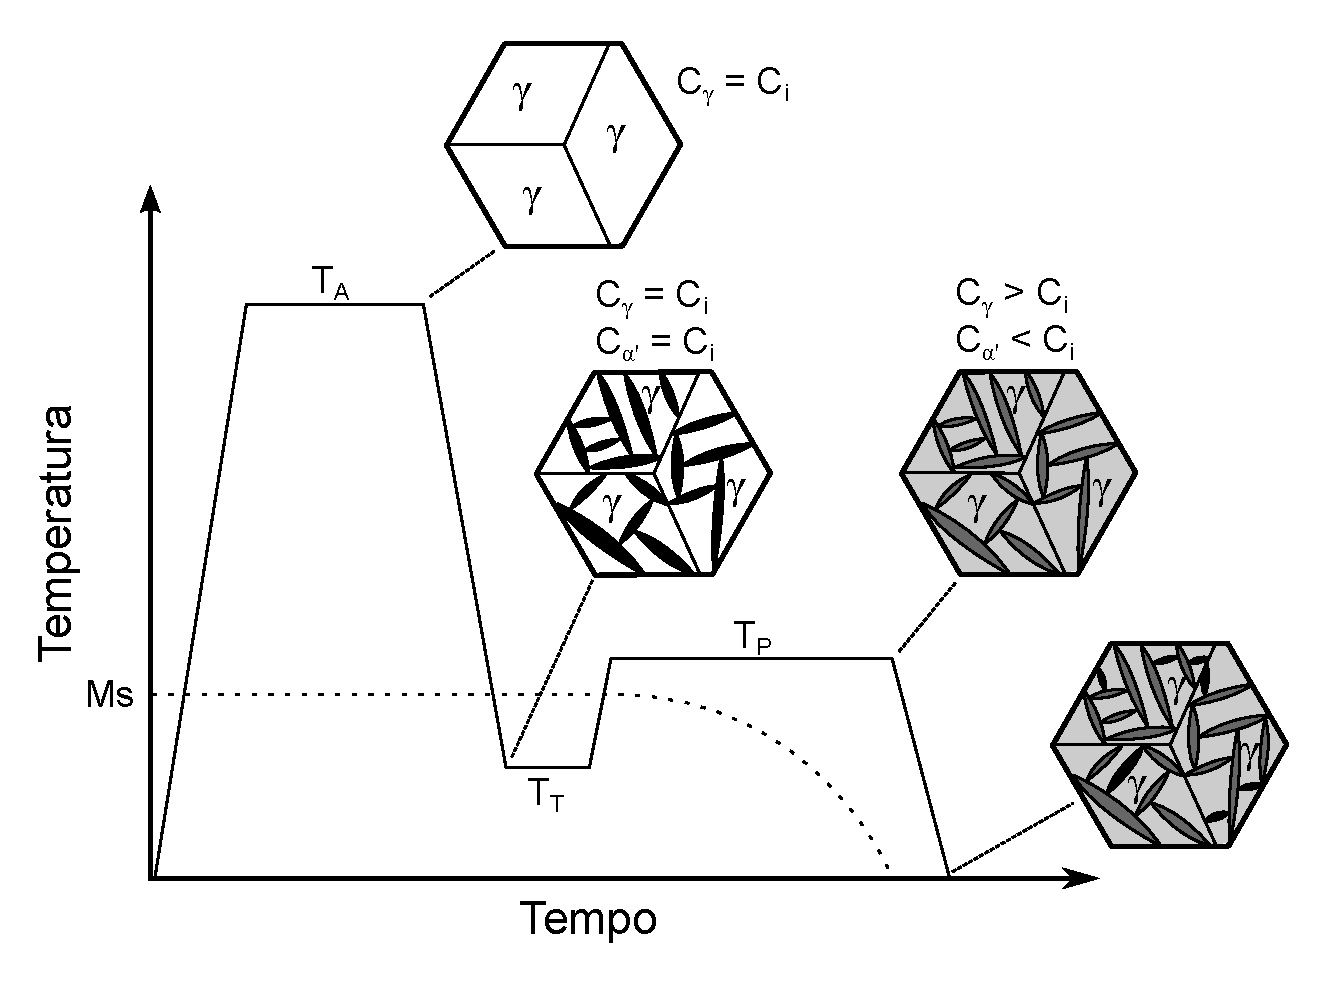
\includegraphics[width=.8\textwidth]{img/Q&P_steel.pdf}
  \end{figure}
\end{frame}

\begin{frame}{Introdução}
  % \only<1>{
  \begin{itemize}
    \item A partição de C de $\alpha'$ para $\gamma$ é termodinamicamente possível devido à diferença de potenciais químicos ($\mu_C^{\alpha'} > \mu_C^\gamma$)
    \item Speer propôs que $\mu_C^{\alpha'}$ e $\mu_C^\gamma$ se igualam após tratamento T\&P
    \item Equilíbrio Constrito de Carbono (ECC): $\mu_C^{\alpha'} = \mu_C^\gamma$  + interface $\alpha'/\gamma$ fixa
    % \item Os teores de C em $\alpha'$ e $\gamma$ são definidos a partir de $\mu_C^{\alpha'} = \mu_C^\gamma$ e das frações iniciais de $\alpha'$ e $\gamma$: Equilíbrio Constrito de Carbono (ECC)
    % \item Assim, C em $\alpha'$ e $\gamma$ depende da fração inicial de $\alpha'$ (depende de $T_T$)
  \end{itemize}

  \begin{figure}
    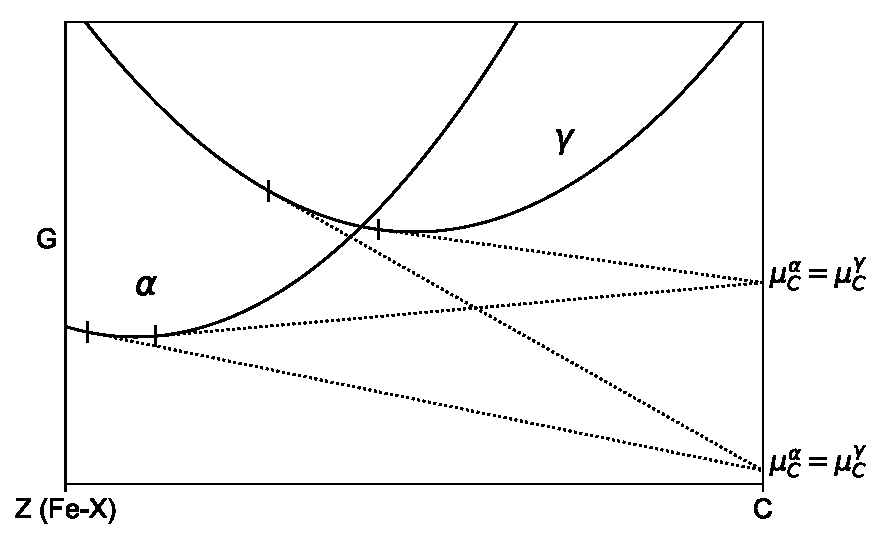
\includegraphics[width=.7\textwidth]{img/common_tangent_CCE.pdf}
  \end{figure}
  % }
  % \only<2>{
  %   \begin{figure}
  %     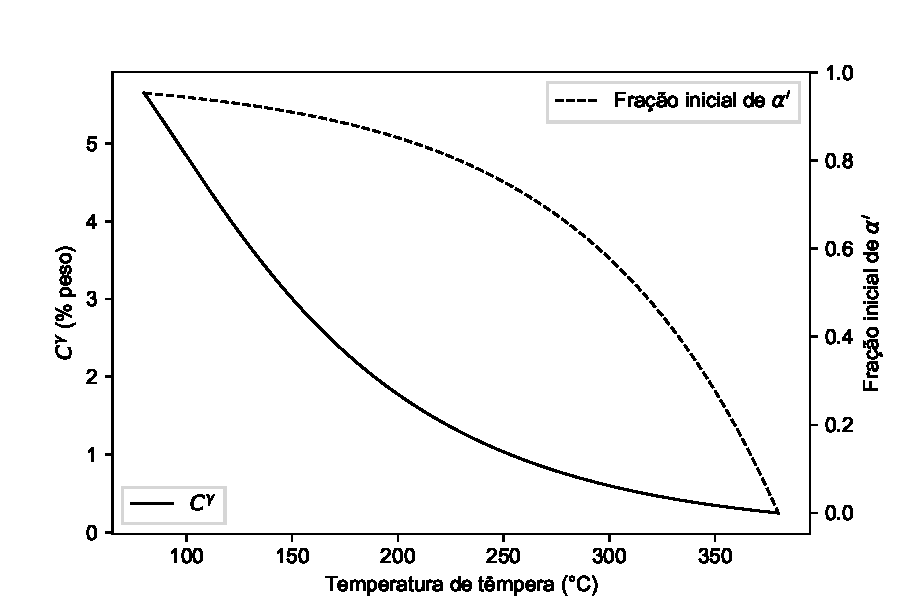
\includegraphics[width=.9\textwidth]{img/CCE_scheme.pdf}
  %   \end{figure}
  % }
\end{frame}

% \begin{frame}
%   \begin{itemize}
%     \item Neste trabalho, a evolução microestrutural e cinética durante a aplicação do processo de \textbf{Têmpera e Partição}\footnotemark[1] (T\&P) de um ferro fundido nodular foi estudada.
%     \item Esta microestrutura promete oferecer propriedades análogas às obtidas durante a transformação bainítica interrompida e aços TRIP e no ferro fundido nodular austemperado (ADI)
%   \end{itemize}
% \end{frame}

%\begin{frame}{Introdução}{Modelo termodinâmico aplicado ao T\&P}
  %\begin{itemize}
    %\item Modelo de Speer (2003): interface $\alpha'$:$\gamma$ imóvel e eq. apenas entre os átomos de C (Equilíbrio Restringido de Carbono - ERC)
    %\item Com base neste modelo, possível determinar \textbf{Temperatura de Têmpera} ótima TO que fornece maior quantidade de austenita
    %\item TT > TO: pouca $\alpha'$ formada, menos carbono para partição para $\gamma$; martensita fresca
    %\item TT < TO: $\gamma$ estabilizado à temperatura ambiente; quantidades menores de $\gamma$ pois é consumido pela formação de $\alpha'$ na têmpera
  %\end{itemize}
%
  %\begin{figure}
  %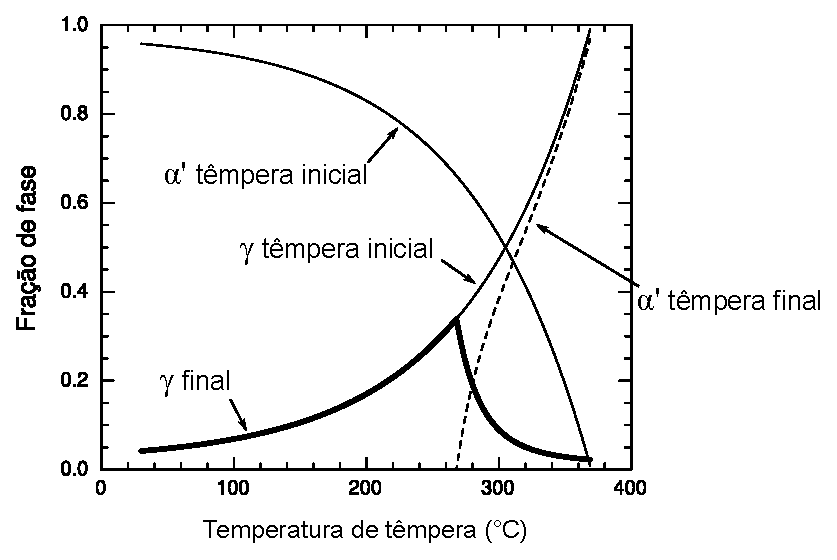
\includegraphics[height=5cm]{../texto/img/TPprevisto.pdf}
  %\end{figure}
%\end{frame}

\begin{frame}{Introdução}
  \begin{block}{Speer, 2004\footnotemark[1]}
    \begin{itemize}
    \item Speer propôs que o elevado teor de Si utilizado na elaboração de ferros fundidos os faria candidatos ótimos para serem submetido à rota T\&P, produzindo microestruturas semelhantes à dos \textbf{ferros fundidos austemperados} (ADI)
    \item Alunos de graduação da Colorado School of Mines, orientados por Speer, submeteram um ferro fundido nodular à rota T\&P e determinaram que o enriquecimento em C de $\gamma$ foi semelhante ao ADI, mas sua retenção foi significativamente menor
    \end{itemize}
  \end{block}

  % \begin{figure}
  % 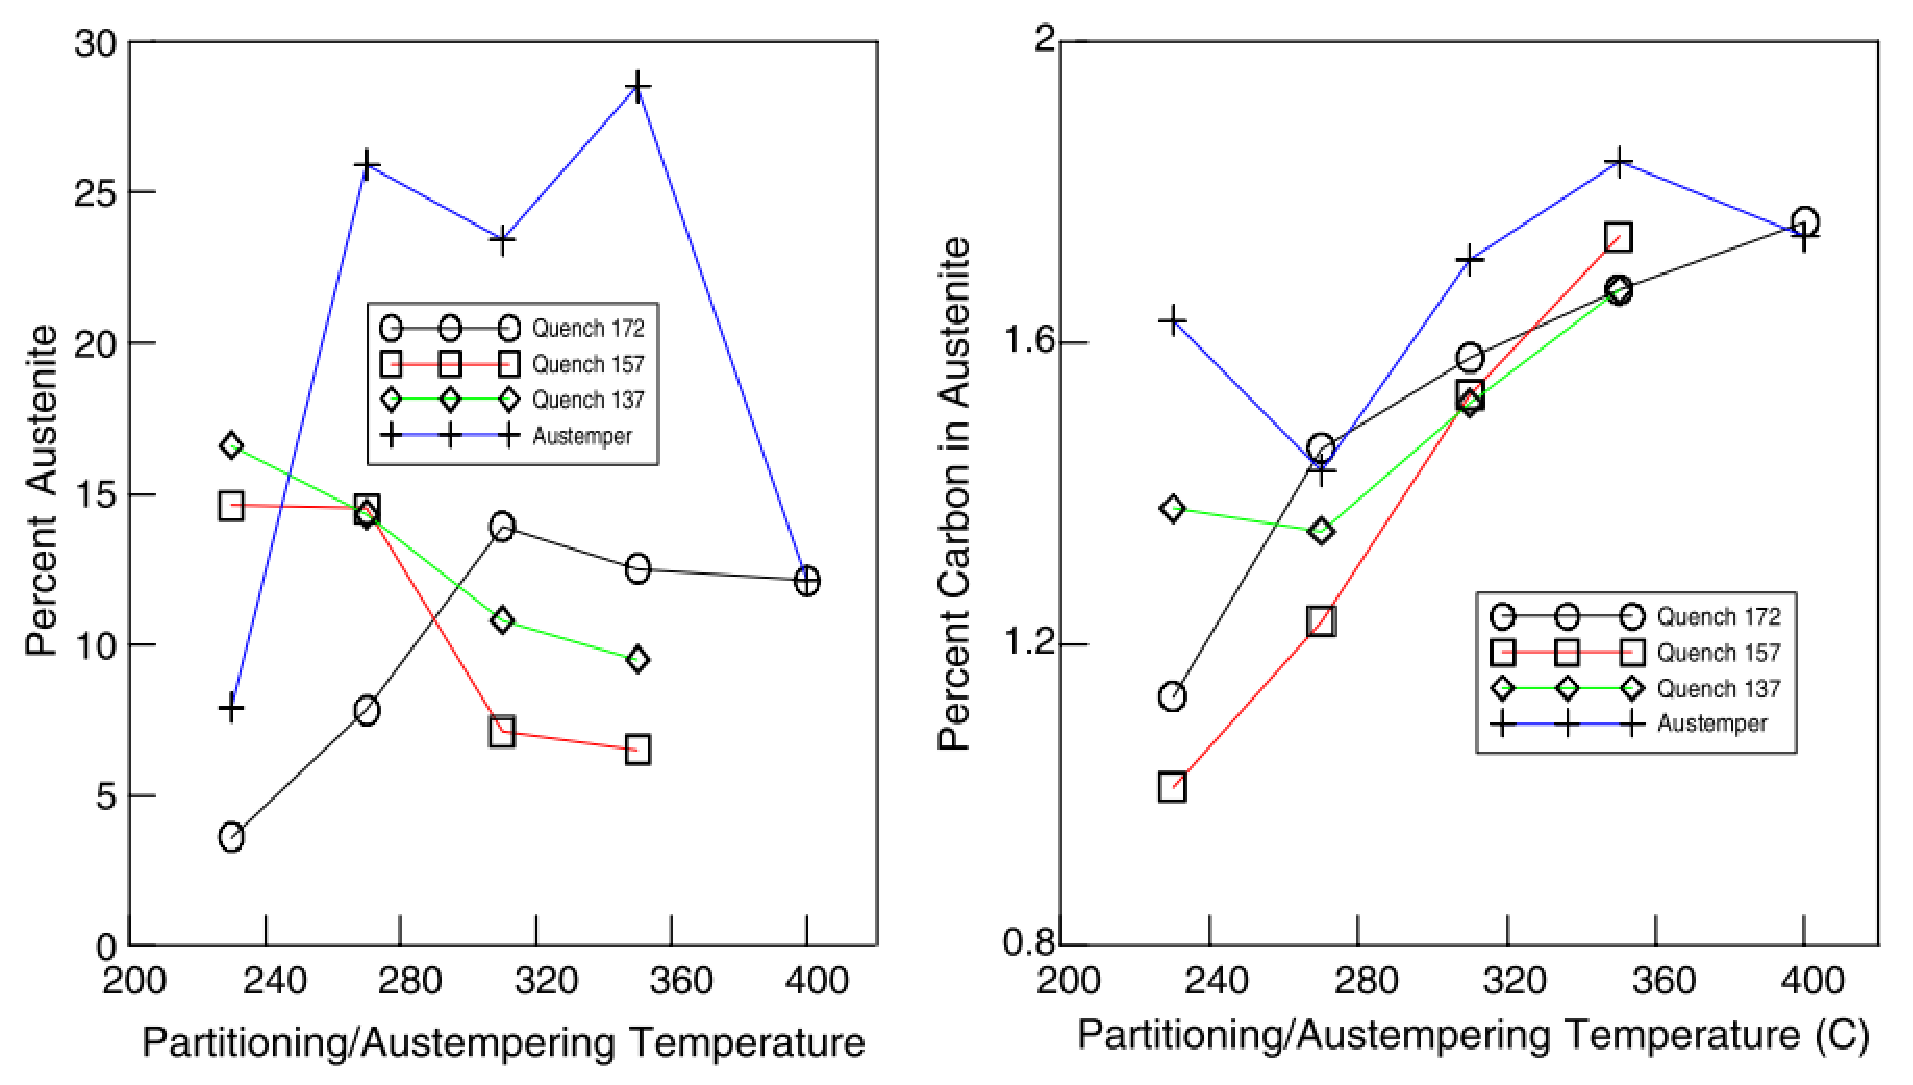
\includegraphics[height=3.8cm]{img/Speer2004.pdf}
  % \end{figure}

  \footnotetext[1]{Speer JG, Edmonds D V., Rizzo FC, Matlock DK. Curr Opin Solid State Mater Sci 2004;8:219.}
\end{frame}

\begin{frame}{Introdução}

  \begin{block}{Dissertação de Anderson J. S. T. Silva\footnotemark[1]}
    \begin{itemize}
    \item Duas ligas comerciais de ferro fundido nodular com alto manganês (> 0,5\%) $\rightarrow$ intensa segregação para contornos de célula eutética
    \item T\&P para diferentes tempos e temperaturas de partição; $T_T$ fixo
    \item Microestrutura composta de $\alpha'$ particionada e grandes quantidades de \textbf{ausferrita} (ferrita bainítica [$\alpha_b$] + $\gamma$), mesmo microconstituinte obtido no ADI
    \item Identificação de \textbf{janela de processo} similar ao ADI, cujo fim é associado ao 2º estágio da reação bainítica
    \end{itemize}

    % \begin{figure}
    %   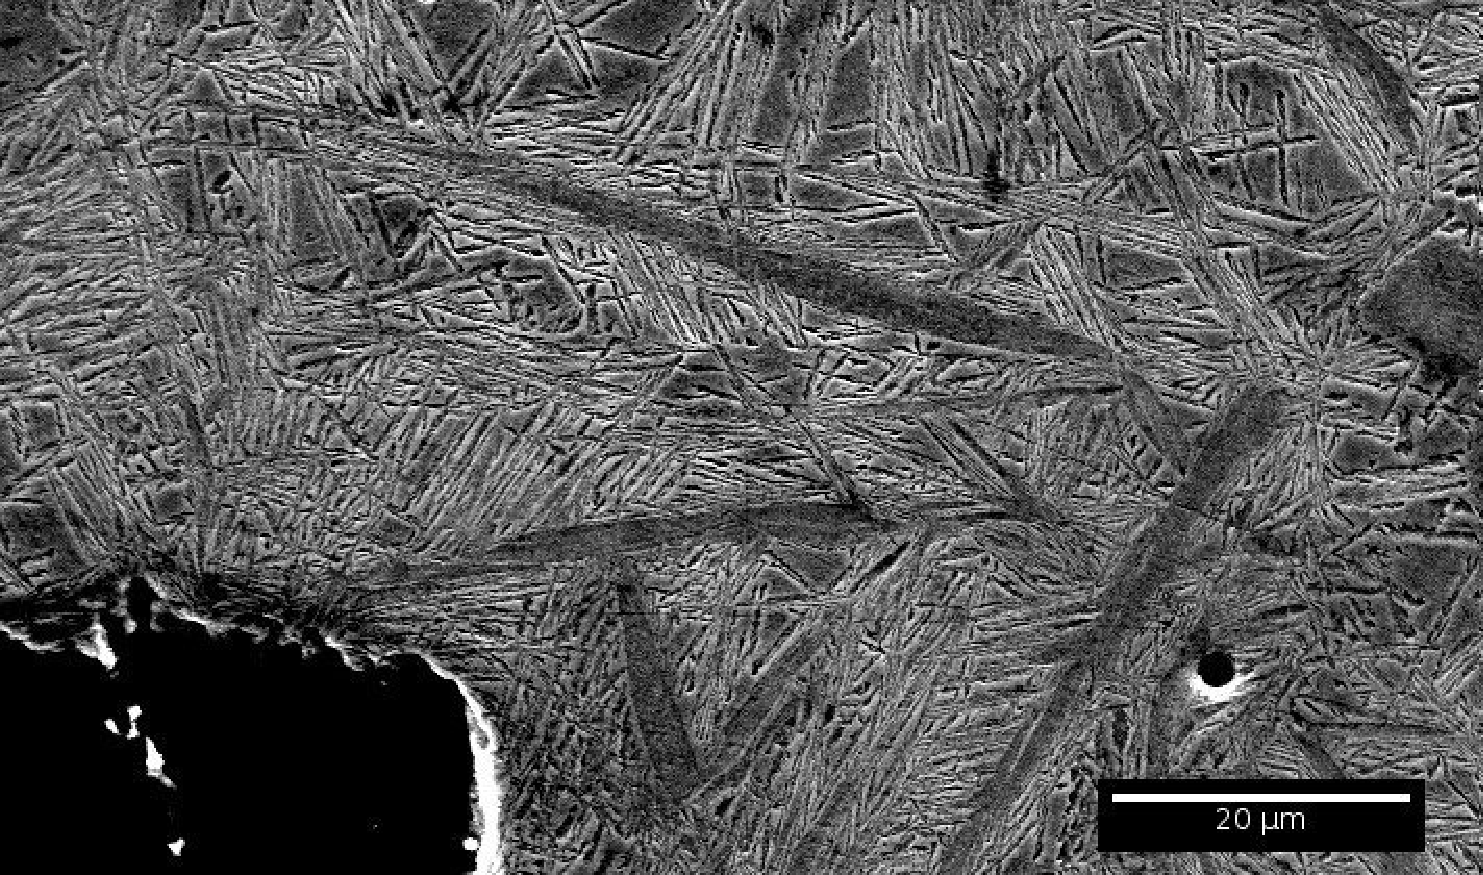
\includegraphics[height=.3\textwidth]{img/MEV_Anderson.pdf}
    % \end{figure}
  \end{block}

  \footnotetext[1]{Silva AJST. Têmpera E Partição de Ferros Fundidos Nodulares. Dissertação (Mestrado). EPUSP, 2013.}
\end{frame}

\begin{frame}{Objetivos}
  Esse trabalho faz parte de um projeto maior que objetiva:
  \begin{enumerate}
    \item Demonstrar a viabilidade da rota T\&P aplicada a ferros fundidos (dissertação de mestrado de Anderson J. S. T. Silva, 2013)
    \item \textbf{Compreender as transformações de fases envolvidas, o entendimento de suas respectivas cinéticas e microestruturas obtidas (presente trabalho)}
    \item Medir as propriedades mecânicas do produto (tese doutorado de André Caetano Melado)
  \end{enumerate}
\end{frame}

% \begin{frame}{Objetivos}
%   \begin{enumerate}
%     \item Avaliar o efeito das variáveis de tratamento térmico na microestrutura final
%     \item Caracterizar a cinética da redistribuição de carbono durante a etapa de partição
%     \item Identificar e caracterizar as reações competitivas que podem ocorrer durante o tratamento de partição, como a reação bainítica e a precipitação de carbonetos
%     \item Avaliar o efeito da microssegregação de elementos de liga, inerente a produtos fundidos, na microestrutura final
%     \item Desenvolver um modelo para a cinética local de redistribuição de carbono durante a etapa de partição, considerando o efeito das reações competitivas.
%   \end{enumerate}
% \end{frame}

% %ADI

% %Equilíbrio Restringido de Carbono


\section{Material e métodos}

\begin{frame}{Material e métodos}{Liga estudada}
  \begin{columns}
    \begin{column}{.6\textwidth}
      \begin{itemize}
        \item Liga fundida como blocos em ``Y'' na Tupy Fundições S.A.
        % \item Microestrutura original ferrítico-perlítica
        \item 3,5\%C, 2,5\%Si, \textbf{0,2\%Mn}, 0,4\%Cu; impurezas (P + S + Cr < 0,1\%)
        \item Inoculação: > 400 nódulos/mm\textsuperscript{2}
      \end{itemize}
    \end{column}

    \begin{column}{.4\textwidth}
      \begin{figure}
        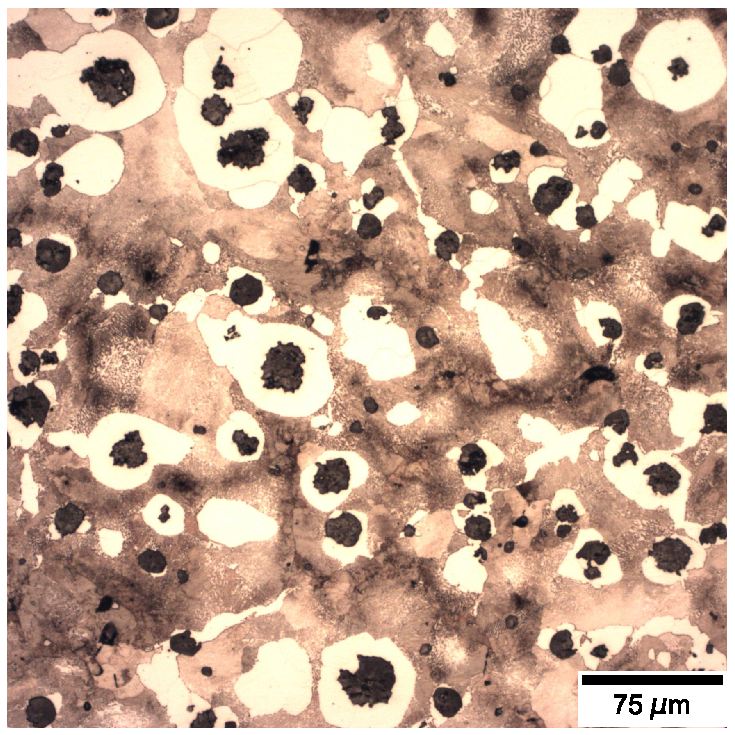
\includegraphics[width=\textwidth]{../tese/img/micrografias/CR/200x-1_scalebar.pdf}
      \end{figure}
    \end{column}
  \end{columns}
\end{frame}

\begin{frame}{Material e métodos}{Dilatometria}
  \begin{itemize}
    \item Dilatômetro Bähr 805A, aquecimento por indução \& resfriamento gás He $\rightarrow$ controle acurado de temperatura
    \item CP cilíndrico \O 4mm, L = 10mm
    \item Aquisição em tempo real da dilatação da amostra $\rightarrow$ cinética de transformação
  \end{itemize}
\end{frame}

\begin{frame}{Material e métodos}{Dilatometria}
  \begin{itemize}
    \item $T_A$ = \SI{880}{\degreeCelsius} no campo $\gamma + grafita$. Thermo-Calc\textregistered{} $\rightarrow$ 0,76\%C em $\gamma$
    \item \textbf{$T_T$ = 140, 170 e 200~\SI{}{\degreeCelsius}}
    \item \textbf{$T_P$ = 300, 375 e 450~\SI{}{\degreeCelsius}}
    \item \textbf{$t_P$ = 0, 30~s, 5~min, 15~min, 2~h}
  \end{itemize}

  \begin{figure}
    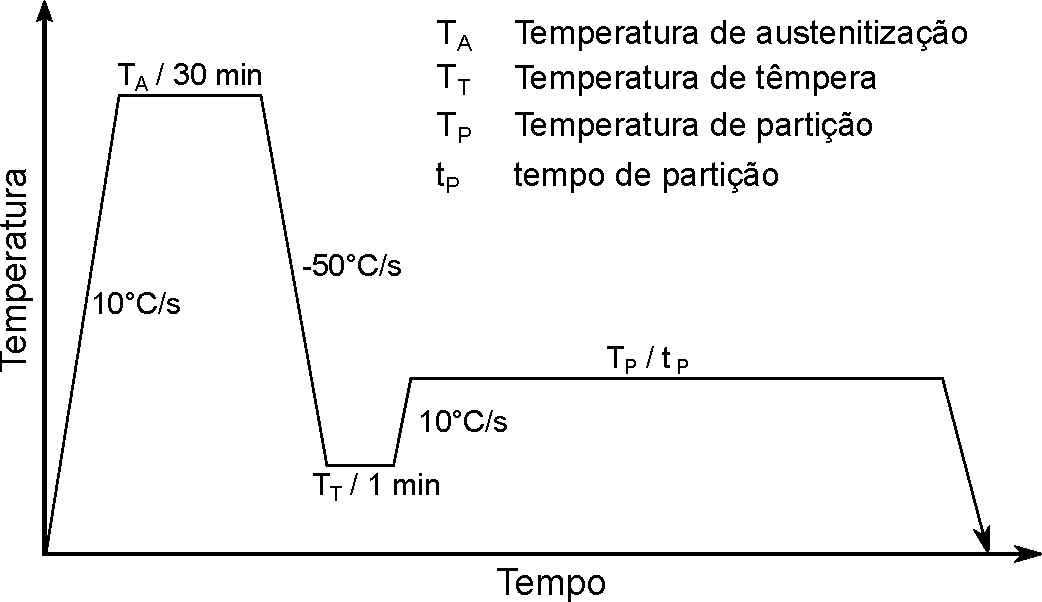
\includegraphics[width=.8\textwidth]{img/expproc_dil.pdf}
  \end{figure}
\end{frame}

\begin{frame}{Difração de raios X in situ}
  \begin{itemize}
    \item XTMS @ LNLS/LNNano: Simulador termomecânico Gleeble\textregistered{} 3S50 + DRX luz síncrotron
    % \item Aquecimento por efeito Joule (passagem de corrente pela amostra)
    \item Aquisição em tempo real de padrões de DRX $\rightarrow$ Evolução de frações de fase e seus respectivos parâmetros de rede
  \end{itemize}

  \begin{figure}
    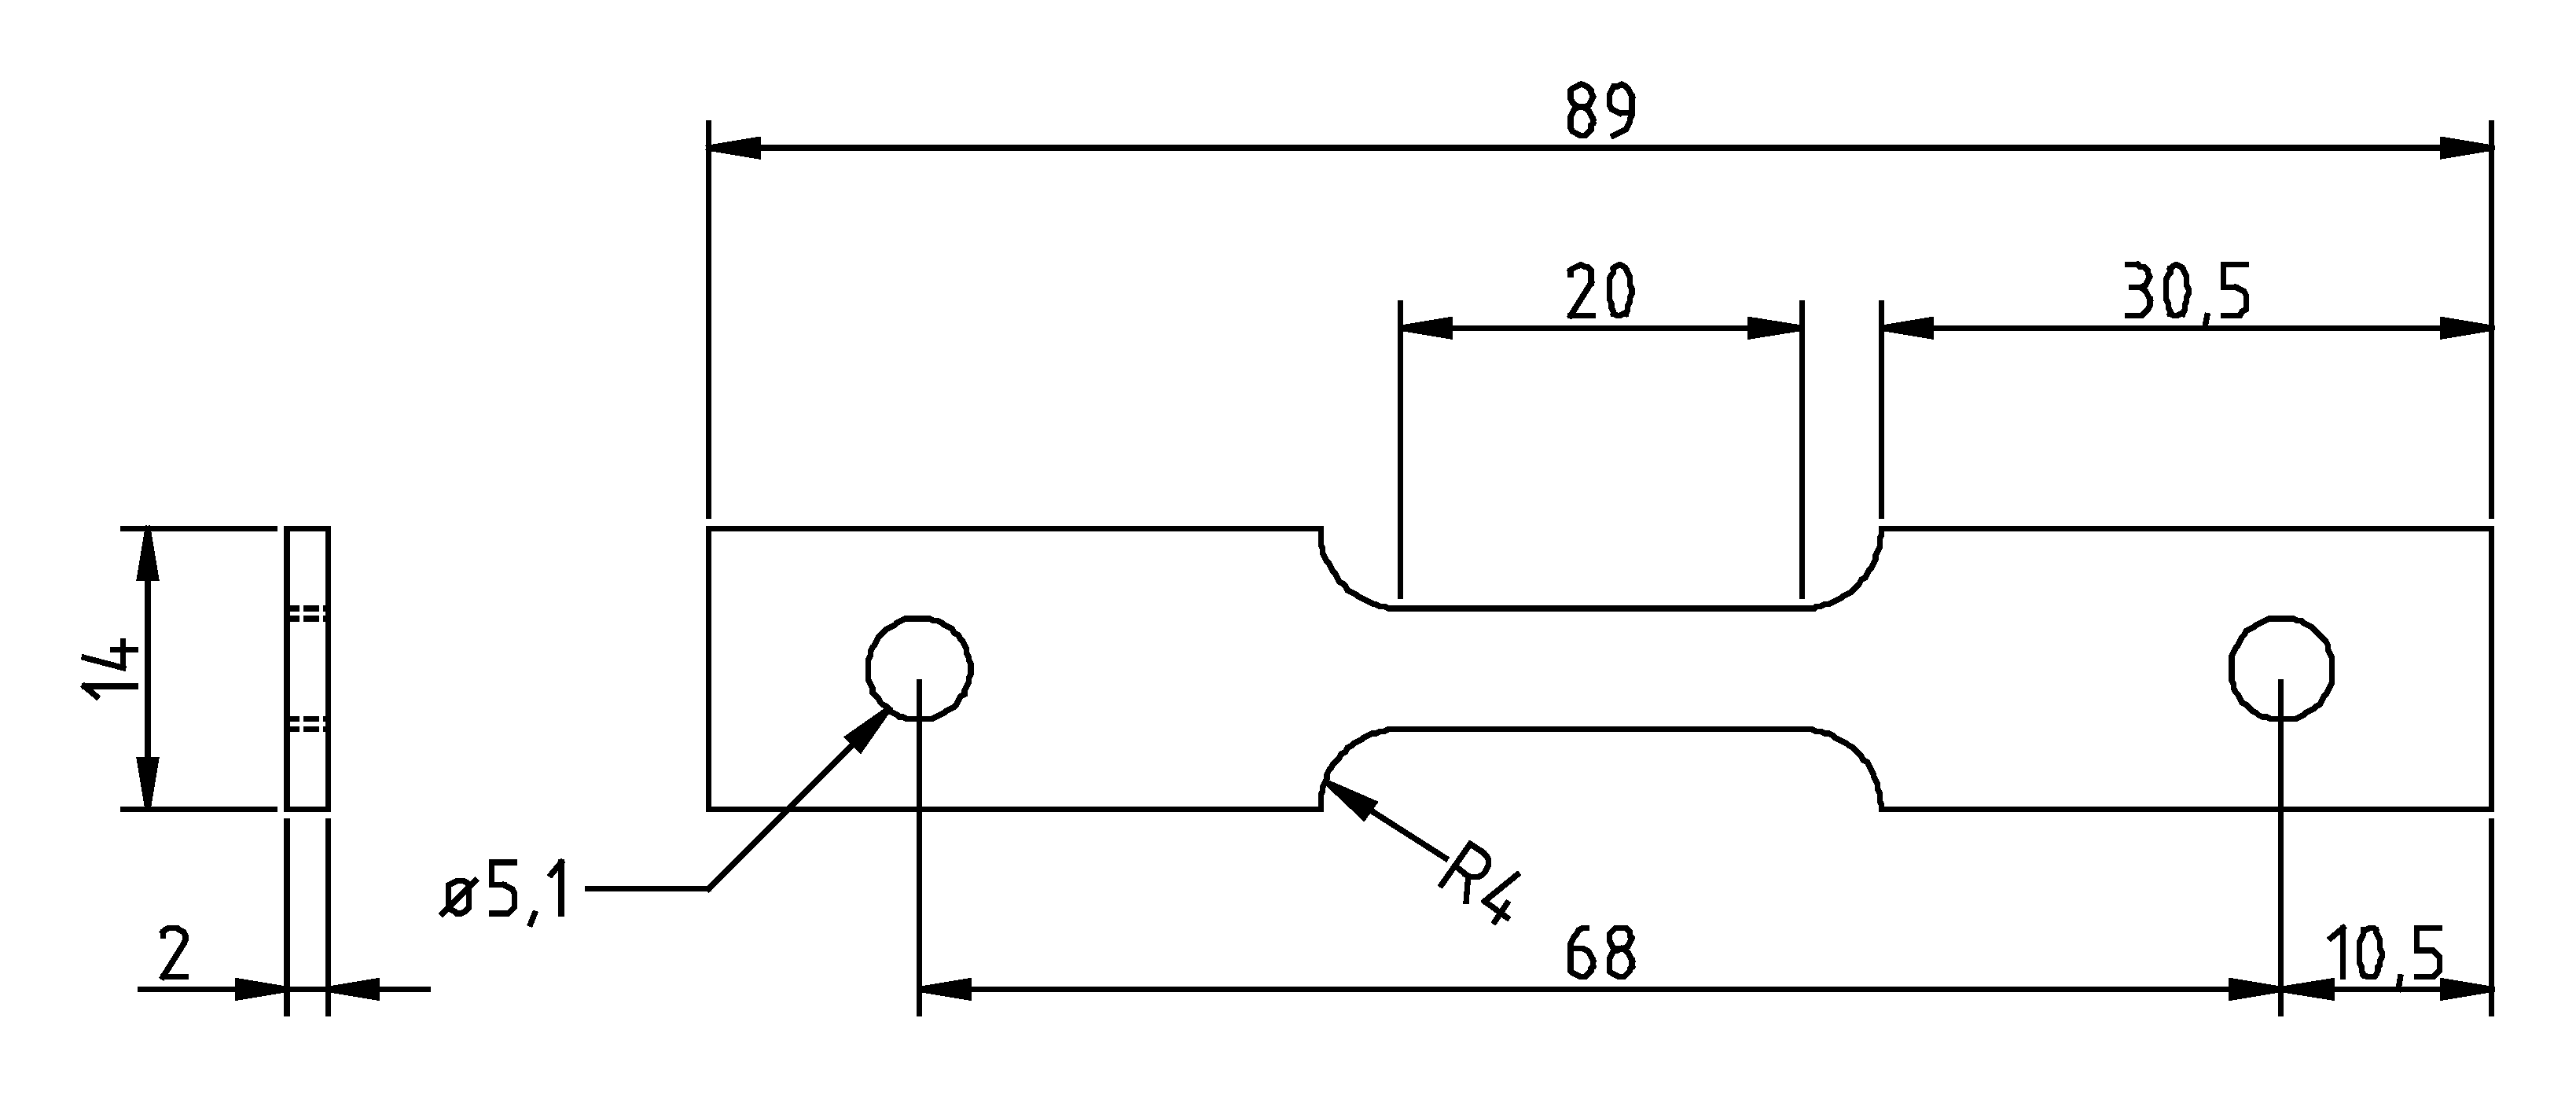
\includegraphics[width=.8\textwidth]{../tese/img/CPXTMS.pdf}
  \end{figure}
\end{frame}

\begin{frame}{Material e métodos}{DRX in situ}
  \begin{itemize}
    \item $T_T$ = \SI{170}{\degreeCelsius}
    \item $T_P$ = 300, 375, \SI{450}{\degreeCelsius} / 2~h

    \item Energia do feixe: 12~keV $\rightarrow \lambda$ = 1,033~\AA
    \item Geometria $\omega-2\theta$; $\omega$ fixo em 15°
    \item Dois detetores multicanal Mythen 1K com 1280 pixels cada
    \item Aquisições: detetores posicionados a 31° $\rightarrow$ 26°--47° (picos (111) e (200) de $\gamma$ e (110) e (200) de $\alpha$); acq. feitas a cada 3,5~s
  \end{itemize}

  \begin{figure}
    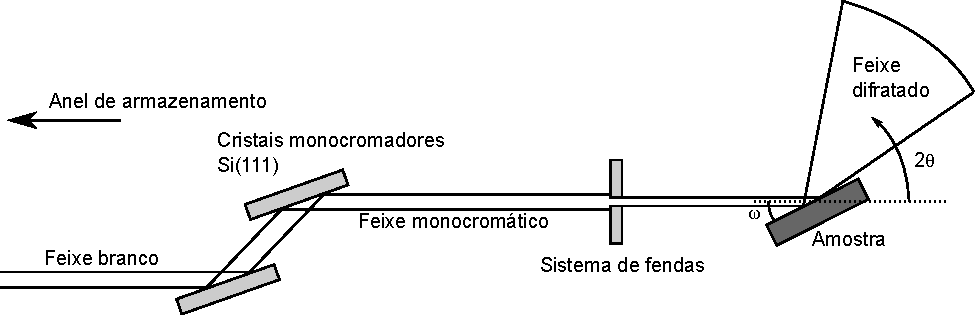
\includegraphics[width=.8\textwidth]{../tese/img/XRD1.pdf}
  \end{figure}
\end{frame}

% \begin{frame}{Material e métodos}{DRX in situ}
%   \begin{figure}
%     \centering
%     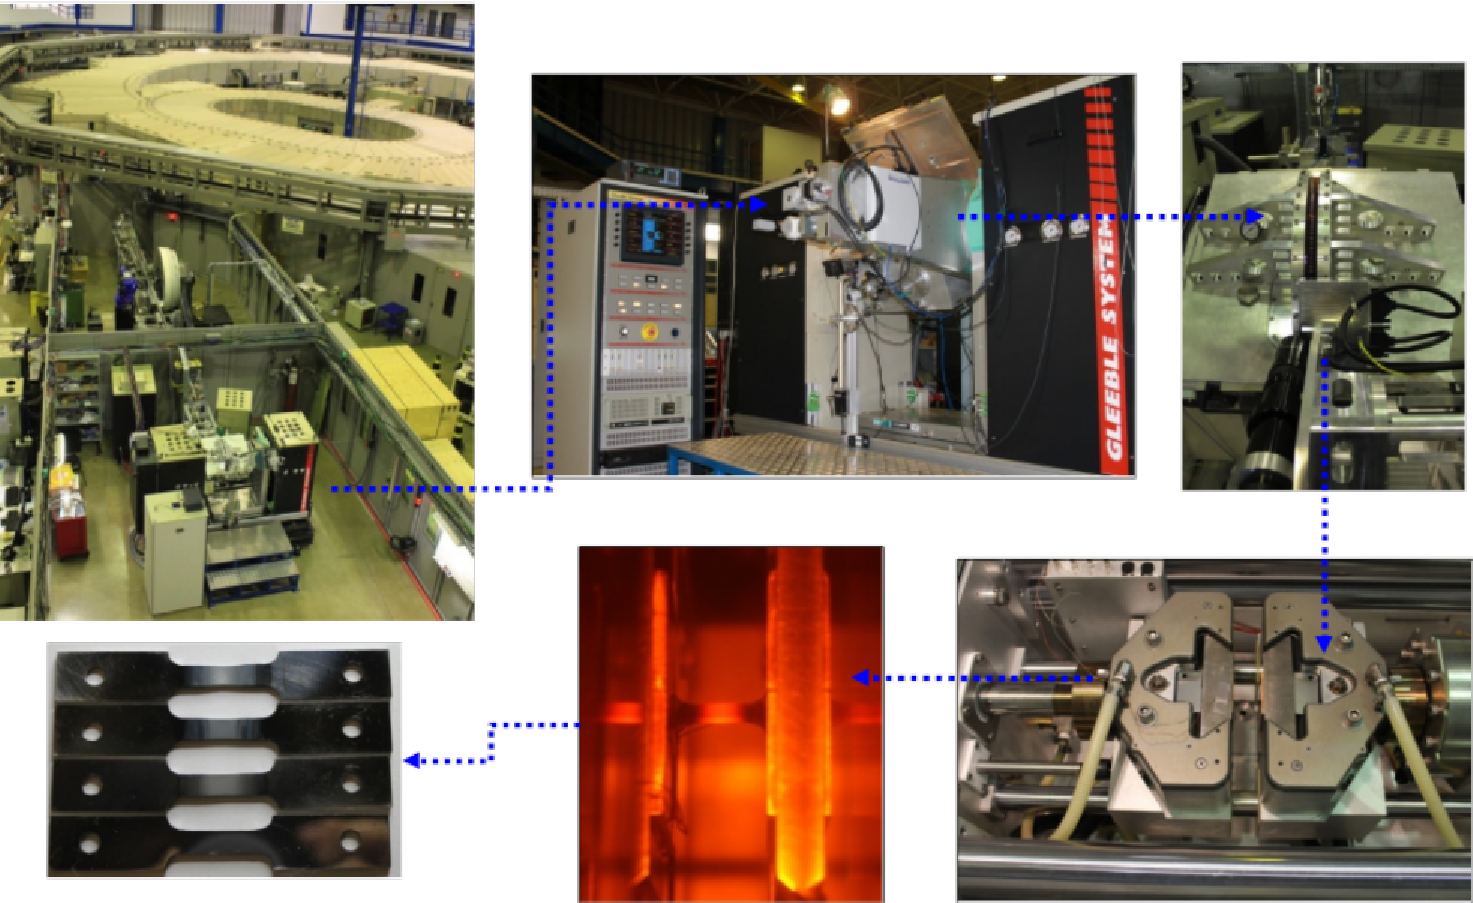
\includegraphics[width=\textwidth]{img/XTMS_facilities.pdf}
%   \end{figure}
% \end{frame}

\begin{frame}{Material e métodos}{DRX in situ}
  Tratamento de dados:
  \begin{itemize}
    \item Quantificação de fases usando procedimento convencional
    \item Determinação do parâmetro de rede da austenita ($a^\gamma$)
    \item Teor de carbono em $\gamma$ estimado pelas equações de van Bohemen\footnotemark[2] Dyson e Holmes\footnotemark[3]

    $$\frac{a^\gamma}{a_0^\gamma} = 1 + B_\gamma T + B_\gamma \Theta_D^\gamma \left[ \exp{\left( -\frac{T}{\Theta_D^\gamma} \right)}\right]$$

    $$a^\gamma = 3,5780 + 3,30\cdot10^{-2} \%w_C^\gamma + 9,5\cdot10^{-4} \%w_{Mn}^\gamma + 1,5\cdot10^{-3} \%w_{Cu}^\gamma$$
  \end{itemize}

  \footnotetext[1]{Stock S, Cullity B. Elements of X-ray diffracion. Prentice Hall, New Jersey, 2001}
  \footnotetext[2]{van Bohemen SMC. Scr Mater 2013;69:315.}
  \footnotetext[3]{Dyson DJ, Holmes B. J Iron Steel Inst 1970;208:469.}
\end{frame}

% \begin{frame}{Material e métodos}{DRX insitu}
%   \tikzset{block/.style={rectangle, draw, text width=15em, rounded corners, minimum width=3.5cm}}
%   \tikzset{title/.style={rectangle, text centered, text width=15em, minimum width=3.5cm, font=\bfseries}}
%   \tikzset{figure/.style={rectangle, text width=20em, minimum width=3.5cm}}
%   \tikzset{line/.style={draw, -latex}}


%   \scalebox{0.55}{
%     \begin{tikzpicture}
%       \node[block,text centered](raw){Dados brutos};
%       \node[block, below=1cm of raw](Gauss){Ajuste dos picos por função de Gauss\footnotemark[1]:\\
%         $I = I_0 \exp{\left[-\left(\frac{2\theta - 2\theta_0}{w}\right)^2\right]}$\alert{ + bck}};
%       \node[block, left=1cm of Gauss](integral){Integração dos picos:\\
%         $A = \int\limits_{-\infty}^{\infty} I_0 \exp{\left[-\left(\frac{2\theta - 2\theta_0}{w}\right)^2\right]} d\theta =$\\
%         $= I_0|w|\sqrt{\pi}$};
%       \node[block, below=1cm of integral](Cullity){Cálculo de $f^\gamma$ pela comparação com intensidades calculadas\footnotemark[2]:\\
%         $f^\gamma = 1 - f^\alpha = \frac{\sum A_{hkl}^\gamma/R_{hkl}^\gamma}{\sum A_{hkl}^\alpha/R_{hkl}^\alpha + \sum A_{hkl}^\gamma/R_{hkl}^\gamma}$};
%       \node[block, right=1cm of Gauss](Bragg){Lei de Bragg $\rightarrow$ converter $2\theta_0$ para $a_{TP}^\gamma$};
%       \node[block, below=1cm of Bragg](correction){Experimentos \textit{in situ} foram feitos na temp. TP $\rightarrow$ transformar $a_{TP}^\gamma$ para $a_{300K}^\gamma$ usando eq. de expansão do reticulado\footnotemark[3]:\\
%         $\frac{\Delta L^\gamma}{L_0^\gamma} = B_\gamma T + B_\gamma \Theta_D^\gamma \left[ \exp{\left( -\frac{T}{\Theta_D^\gamma} \right)}\right]$\\
%         em que $B_\gamma=24,8\times 10^{-1} K^{-1}$ e $\Theta_D^\gamma=280 K$};
%       \node[block, below=1cm of correction](Dyson){Computar teor de carbono utilizando relação entre $a^\gamma$ e $\%w_C^\gamma$ de Dyson e Holmes\footnotemark[4]:\\
%         $a^\gamma = 3,5780 + 3,30\cdot10^{-2} \%w_C^\gamma + 9,5\cdot10^{-4} \%w_{Mn}^\gamma + 1,5\cdot10^{-3} \%w_{Cu}^\gamma$};
%       \node[figure, below=0.5cm of Gauss]{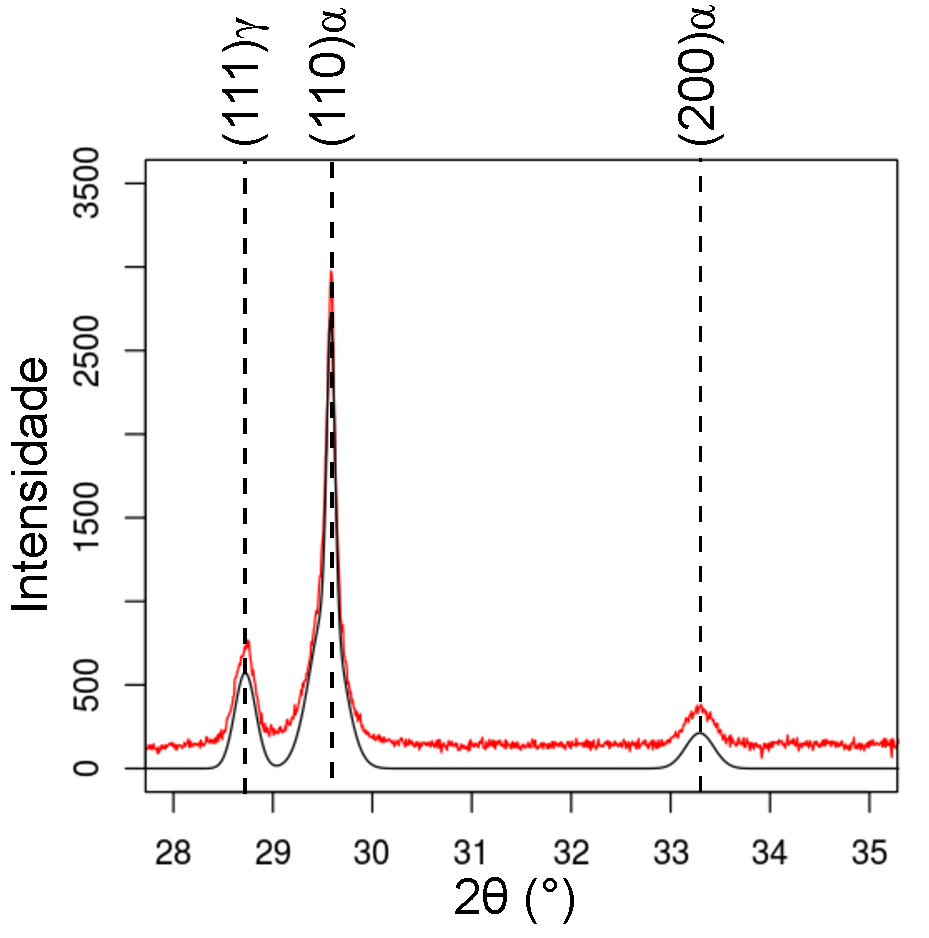
\includegraphics[width=20em]{img/peak_fitting.pdf}};
%       \node[title, above=0.5cm of integral]{Cálculo das frações volumétricas de $\alpha$ e $\gamma$};
%       \node[title, above=0.5cm of Bragg]{Cálculo do teor de carbono em $\gamma$};

%       \path[line](raw) -- (Gauss);
%       \path[line](Gauss) -- (integral);
%       \path[line](integral) -- (Cullity);
%       \path[line](Gauss) -- (Bragg);
%       \path[line](Bragg) -- (correction);
%       \path[line](correction) -- (Dyson);
%     \end{tikzpicture}
%   }
%   \footnotetext[1]{Babu SS, Specht ED, David SA, Karapetrova E, Zschack P, Peet M, Bhadeshia HKDH. Metall Mater Trans A 2005;36:3281.}
%   \footnotetext[2]{Stock S, Cullity B. Elements of X-ray diffracion. Prentice Hall, New Jersey, 2001}
%   \footnotetext[3]{van Bohemen SMC. Scr Mater 2013;69:315.}
%   \footnotetext[4]{Dyson DJ, Holmes B. J Iron Steel Inst 1970;208:469.}

% \end{frame}


\begin{frame}{Material e métodos}{Caracterização microestrutural}
  \begin{itemize}
    \item \textbf{MO}: Olympus BX60M (PMT-USP) e microscópio Nikkon (Tohoku University)
    \item \textbf{MEV}: MEV-FEG FEI Inspect F50 (PMT-USP) e JEOL JSM-7001F (Tohoku University)
    
    \begin{itemize}
      \item Preparação metalográfica convencional por lixamento e polimento até sílica coloidal
      \item MO e MEV: Ataque metalográfico com reagente Nital 2\%
    \end{itemize}

    \item \textbf{EBSD} (difração de elétrons retroespalhados): JEOL JSM-7001F com sistema TSL OIM (Tohoku University)

    \item \textbf{EPMA} (microssonda eletrônica): JEOL JXA-FE-8530 (IGc-USP)
    
    \begin{itemize}
      \item Baixo aumento: análise composicional de Mn, Si e Cu (C é estimado usando termodinâmica computacional)
      \item Alto aumento: análise composicional de C
    \end{itemize}
  \end{itemize}
\end{frame}

\begin{frame}{Material e métodos}{Difração de raios X de alta resolução}
  \begin{itemize}
    \item DRX síncrotron feita na XTMS, mas sem tratamento térmico
    \item Detetor 2D Rayonix SX165: alta resolução, alto sinal/ruído $\rightarrow$ \emph{Caracterização de carbonetos}
    \item Dados integrados azimutalmente $\rightarrow$ difratograma 1D
  \end{itemize}

  % \only<1>{
  %   \begin{figure}
  %     \begin{minipage}[c][.5\textwidth]{0.35\textwidth}%
  %     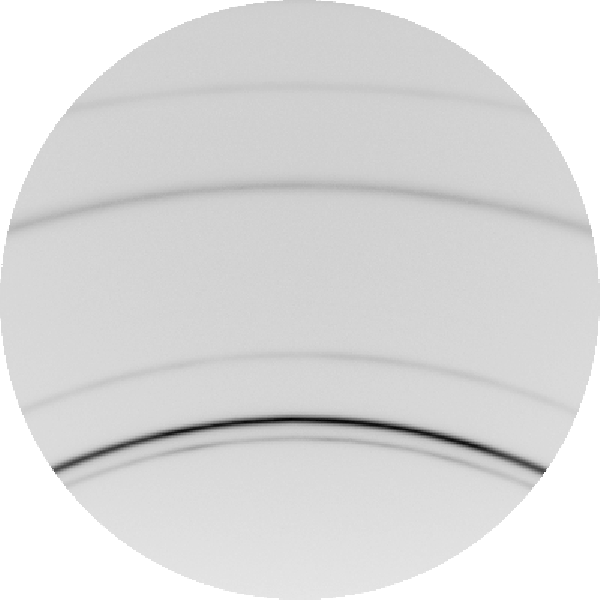
\includegraphics[width=\textwidth]{../tese/img/XTMS/PT300_detector.pdf}
  %     \end{minipage}\hfill
  %     \begin{minipage}[c][.5\textwidth]{0.6\textwidth}%
  %     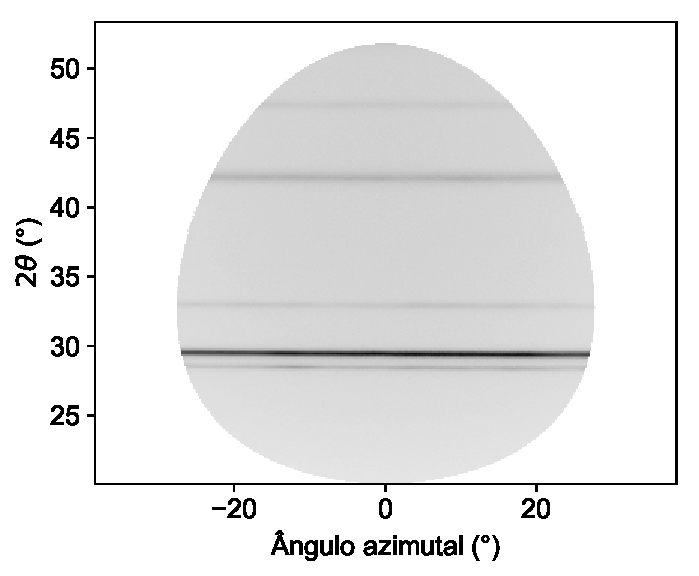
\includegraphics[width=\textwidth]{../tese/img/XTMS/PT300_spherical.pdf}
  %     \end{minipage}
  %   \end{figure}
  % }
  % \only<2>{
  %   \begin{figure}
  %     \subfloat{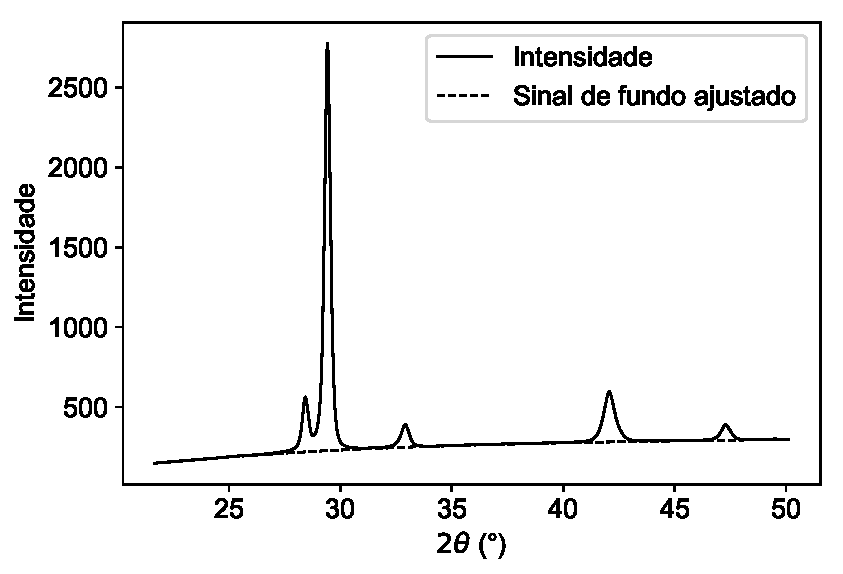
\includegraphics[width=.7\textwidth]{../tese/img/XTMS/PT300_diffractogram.pdf}}
  %   \end{figure}
  % }
\end{frame}

\section{Resultados e discussão}

\AtBeginSubsection[]{
  \begin{frame}<beamer>{Sumário}
    \tableofcontents[currentsection,currentsubsection]
  \end{frame}
}

\AtBeginSubsubsection[]{
  \begin{frame}<beamer>{Sumário}
    \tableofcontents[currentsection,currentsubsection,currentsubsubsection]
  \end{frame}
}

%%%%%%%%%%%%%%%%%%%%%%%%%%%%%%%%%%%%%%%%%%

\subsection{Características microestruturais pré etapa de partição}

\begin{frame}{Transformação martensítica}
  \only<1>{
    \begin{figure}
      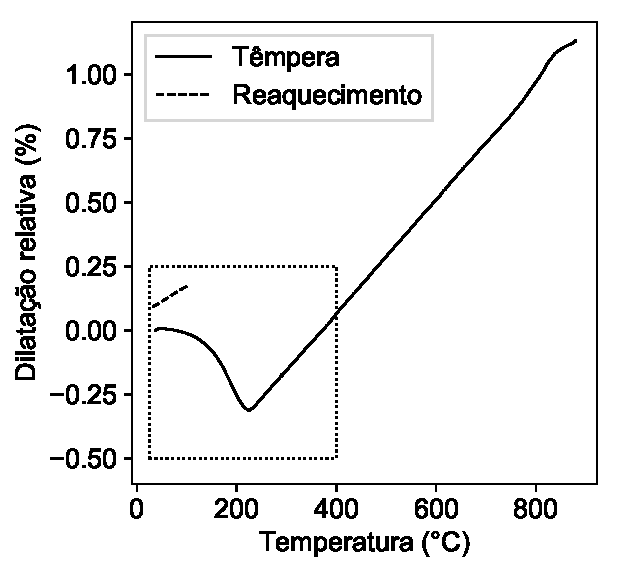
\includegraphics[width=.8\textwidth]{../tese/img/dilatometria/dil_martensita.pdf}
    \end{figure}
  }
  \only<2>{
    \begin{columns}
      \begin{column}{.6\textwidth}
        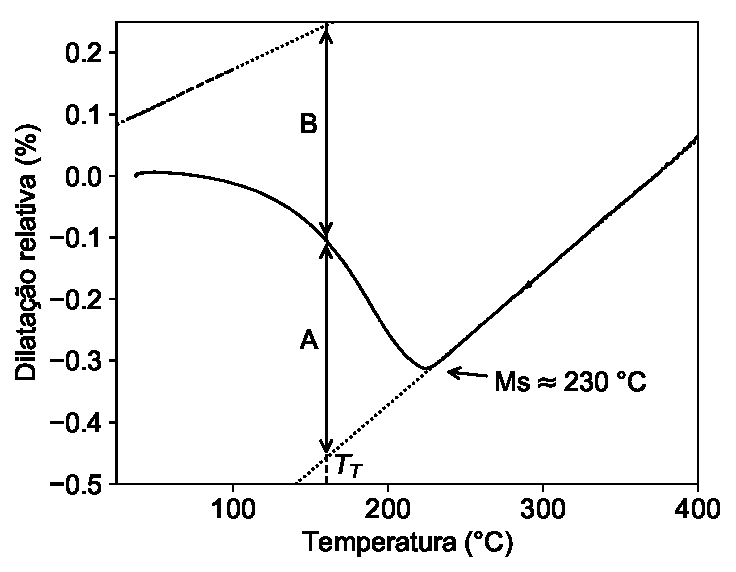
\includegraphics[width=\textwidth]{../tese/img/dilatometria/dil_martensita_close.pdf}
      \end{column}

      \begin{column}{.4\textwidth}
          Regra das alavancas:

          $$f^{\alpha'} = 1 - f^\gamma = \frac{A}{A + B}$$
      \end{column}
    \end{columns}
  }
\end{frame}

\begin{frame}{Transformação martensítica}
  $$f^{\alpha'} = 1 - f^\gamma = 1 - \exp\left[ -1,217 \times 10^{-2} \left( 216,2 - T_T \right) \right]$$

  \only<1>{
    \begin{figure}
      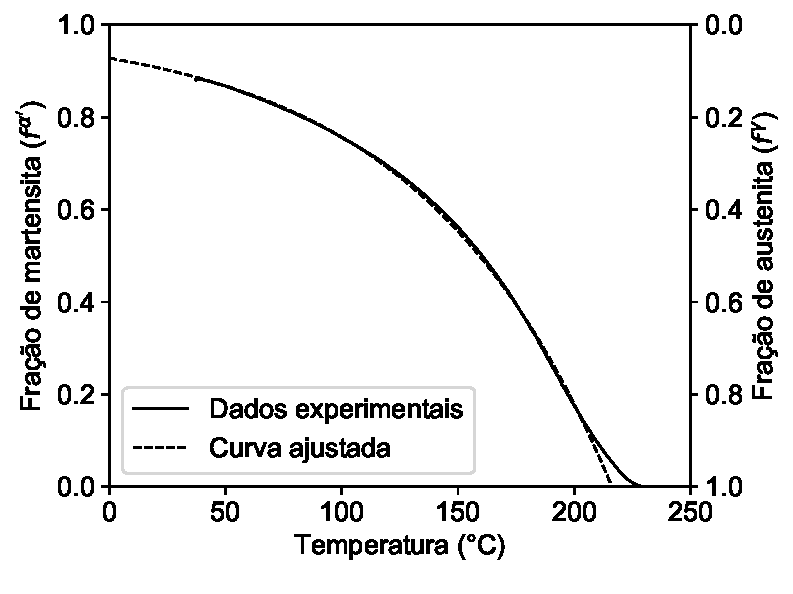
\includegraphics[width=.8\textwidth]{../tese/img/dilatometria/frac_martensita.pdf}
    \end{figure}
  }

  \only<2>{
    \begin{table}
      \begin{tabular}{c c c}
      \hline
      $T_T$ (°C) & $f^{\alpha'}$ (\% vol) & $f^\gamma$ (\% vol)\\
      \hline
      25 &  90,2 & 9,8\\
      140 & 60,4 & 39,6\\ 
      170 & 43,0 & 57,0\\
      200 & 17,9 & 82,1\\
      \hline
      \end{tabular}
    \end{table}
  }
\end{frame}

\begin{frame}{Transformação martensítica}
  $T_T = \SI{170}{\degreeCelsius} / \SI{1}{min}$ ($f^{\alpha'}$ = 43,0\%)

  \begin{figure}
    \includegraphics<1>[width=.8\textwidth]{img/TT170.pdf}
  \end{figure}
\end{frame}

\begin{frame}{Transformação martensítica}
  $T_T = \SI{170}{\degreeCelsius} / \SI{1}{min}$ ($f^{\alpha'}$ = 43,0\%)
  \begin{itemize}
    \item Martensita levemente revenida $\rightarrow$ atacada pelo Nital
    \item Áreas brancas / alto relevo: \textbf{austenita ($\gamma$)} não transformada após $\SI{170}{\degreeCelsius} / \SI{1}{min}$ $\rightarrow$ transforma-se parcialmente em \textbf{martensita fresca ($\alpha_{fr}'$)} durante resfriamento final
    \item \textbf{$\alpha_{fr}' + \gamma$: MA}
  \end{itemize}

  \begin{figure}
    \includegraphics<1>[width=.5\textwidth]{../tese/img/micrografias/Q170-1min/500x-1.pdf}
    \includegraphics<2>[width=.5\textwidth]{../tese/img/micrografias/Q170-1min/5kx-4_scalebar.pdf}
  \end{figure}
\end{frame}

\begin{frame}{Microssegregação}
  \begin{itemize}
    \item EPMA: composição medida de Mn, Si e Cu
    \item C calculado assumindo potencial químico homogêneo a 880~°C
  \end{itemize}

  \begin{figure}
    \includegraphics<1>[width=.7\textwidth]{../tese/img/EPMA/EPMA.pdf}
  \end{figure}
\end{frame}
  
% \begin{frame}{Microssegregação}
%   Simulação Scheil mostra mesma tendência de segregação

%   \begin{figure}
%     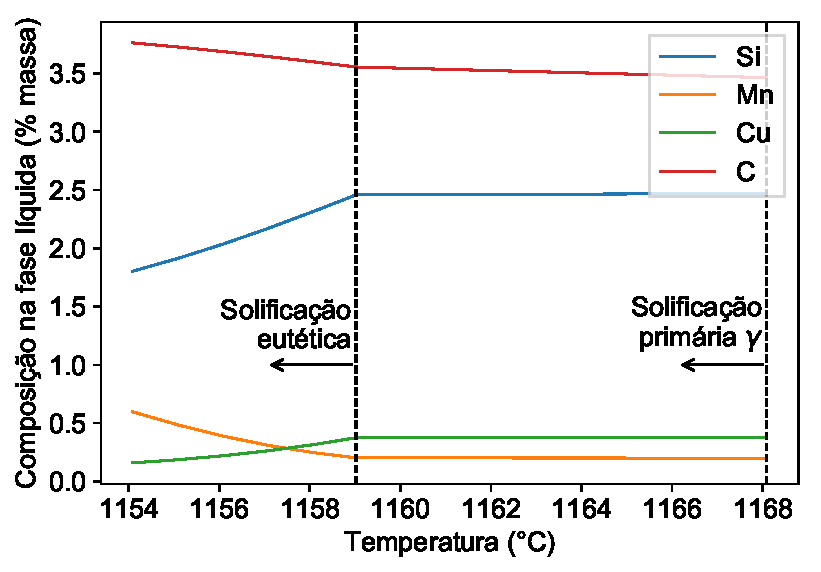
\includegraphics[width=.8\textwidth]{../tese/img/thermo-calc/scheil.pdf}
%   \end{figure}
% \end{frame}

\begin{frame}{Distribuição esperada da martensita}
  Ms calculado ponto a ponto:

  $$\textcolor{red}{Ms}\,\text{(°C)} = 565 - 600 \left[1 - \exp \left( -0.96 w_C^\gamma \right)\right] - 31 w_{Mn}^\gamma - 13 w_{Si}^\gamma$$

  A partir do Ms calculado, é determinada $f^{\alpha'}$ ponto a ponto pela equação de Koistinen-Marburger:

  $$f^{\alpha'} = 1 - \exp\left[ -1,217 \times 10^{-2} \left( \textcolor{red}{Ms} - T_T \right) \right]$$
\end{frame}

\begin{frame}{Distribuição esperada da martensita}
  $T_T = \SI{170}{\degreeCelsius}$

  \begin{figure}
    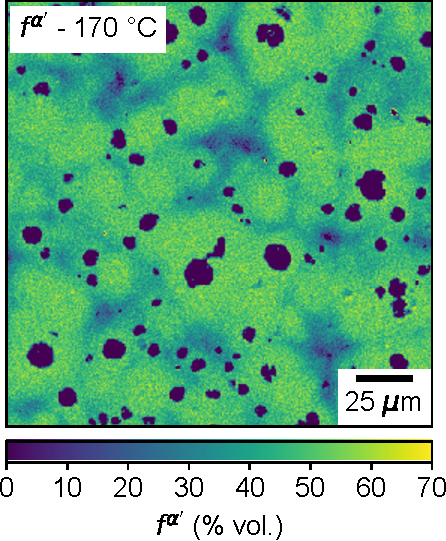
\includegraphics[width=.49\textwidth,valign=t]{img/fmart_TQ170.pdf}\hfill
    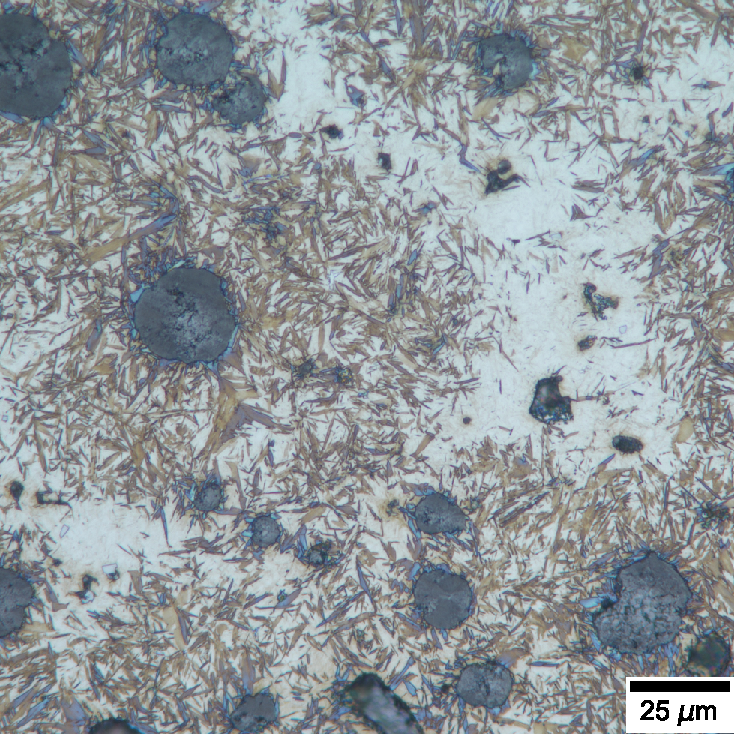
\includegraphics[width=.49\textwidth,valign=t]{../tese/img/micrografias/Q170-1min/500x-1.pdf}
  \end{figure}
\end{frame}

\begin{frame}{Distribuição esperada da martensita}
  \begin{itemize}
    \item $T_T = 25,\ 140,\ 170,\ \SI{200}{\degreeCelsius}$
    \item Histogramas da distribuição de $f^{\alpha'}$ calculada pelo método anterior
    \item Distribuição de martensita fica mais homogênea quanto a temperatura de têmpera é diminuída.
  \end{itemize}

  \begin{figure}
    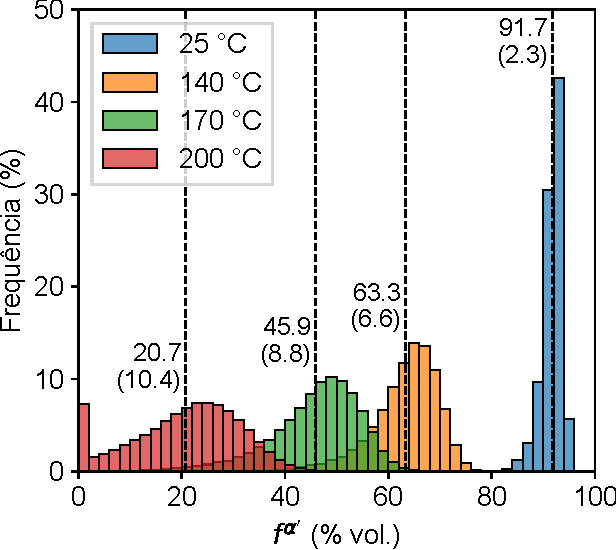
\includegraphics[width=.7\textwidth]{img/fmart_different_TQ.pdf}\hfill
  \end{figure}
\end{frame}

%%%%%%%%%%%%%%%%%%%%%%%%%%%%%%%%%%%%%%%%%%

\subsection{Caracterização microestrutural das amostras T\&P}

% \begin{frame}{Microestruturas T\&P}{Efeito do tempo de partição ($t_P$)}
%   $T_T = \SI{170}{\degreeCelsius}$; $T_P = \SI{375}{\degreeCelsius}$
  
%   \begin{itemize}
%     \item Áreas brancas: austenita não transformada na etapa de partição
%     \item<3> Tempos longos: austenita é consumida (bainita?)
%   \end{itemize}

%   \only<1>{
%     \begin{figure}
%       \subfloat[$t_P = 0$]{\includegraphics[width=.49\textwidth]{../tese/img/micrografias/170-375/MO/QP0_scalebar.pdf}}\hfill
%       \subfloat[$t_P = 30~s$]{\includegraphics[width=.49\textwidth]{../tese/img/micrografias/170-375/MO/QP30s_scalebar.pdf}}
%     \end{figure}
%   }
%   \only<2>{
%     \begin{figure}
%       \subfloat[$t_P = 0$]{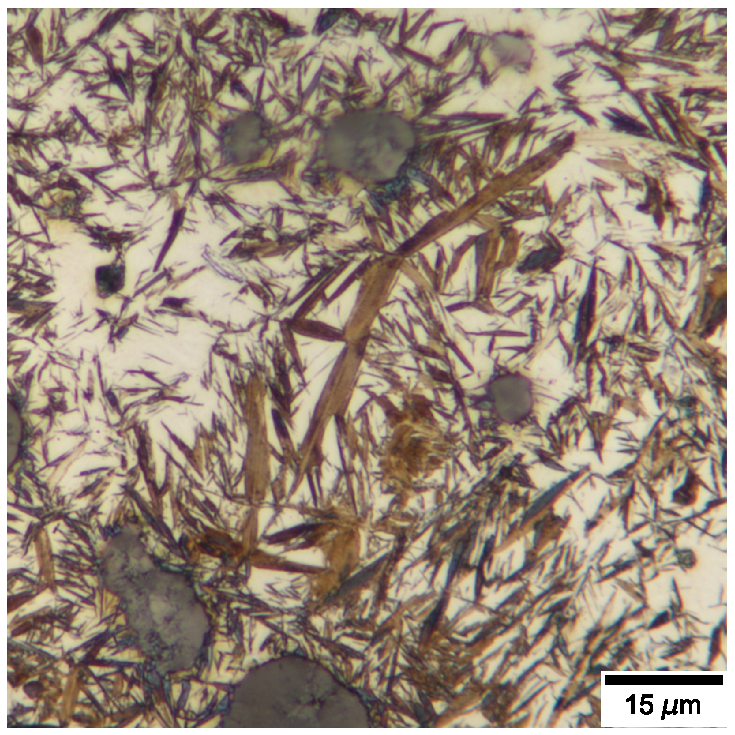
\includegraphics[width=.49\textwidth]{../tese/img/micrografias/170-375/MO/QP0_1000x_scalebar.pdf}}\hfill
%       \subfloat[$t_P = 30~s$]{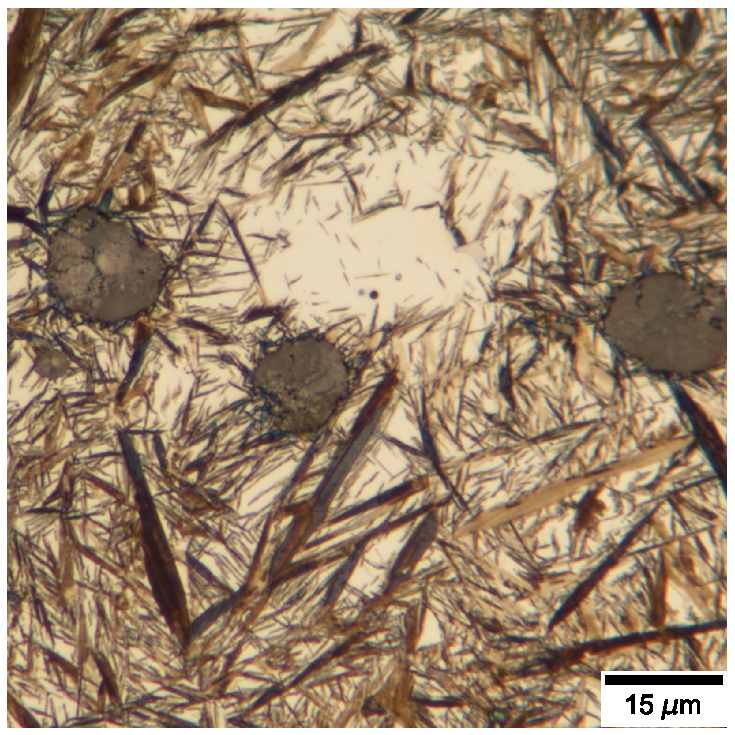
\includegraphics[width=.49\textwidth]{../tese/img/micrografias/170-375/MO/QP30s_1000x_scalebar.pdf}}
%     \end{figure}
%   }
%   \only<3>{
%     \begin{figure}
%       \subfloat[$t_P = 5~min$]{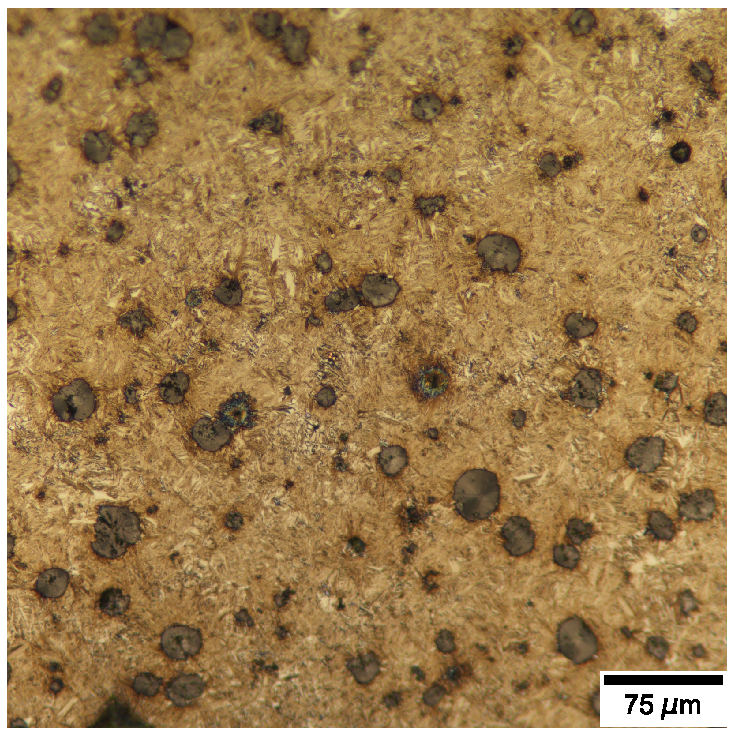
\includegraphics[width=.49\textwidth]{../tese/img/micrografias/170-375/MO/QP5min_scalebar.pdf}}\hfill
%       \subfloat[$t_P = 15~min$]{\includegraphics[width=.49\textwidth]{../tese/img/micrografias/170-375/MO/QP15min_scalebar.pdf}}
%     \end{figure}
%   }
% \end{frame}

\begin{frame}{Microestruturas T\&P}{Efeito do tempo de partição ($t_P$)}
  $T_T = \SI{170}{\degreeCelsius}$; $T_P = \SI{375}{\degreeCelsius}$ / 0

  \begin{itemize}
      % \item Áreas brancas em MO $\rightarrow$ alto relevo em MEV
      \item Padrão de ataque releva carbonetos ($\theta$) no tempo mais curto
      \item $\theta$ portanto se forma no aquecimento de $T_T$ a $T_P$
  \end{itemize}

  \begin{figure}
    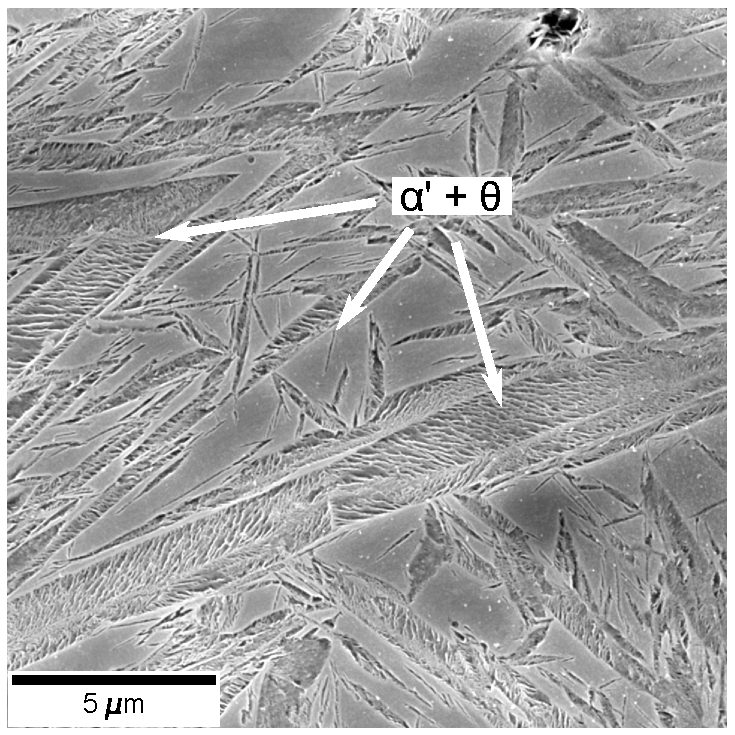
\includegraphics[width=.49\textwidth]{../tese/img/micrografias/170-375/MEV/0/5kx-3.pdf}\hfill
    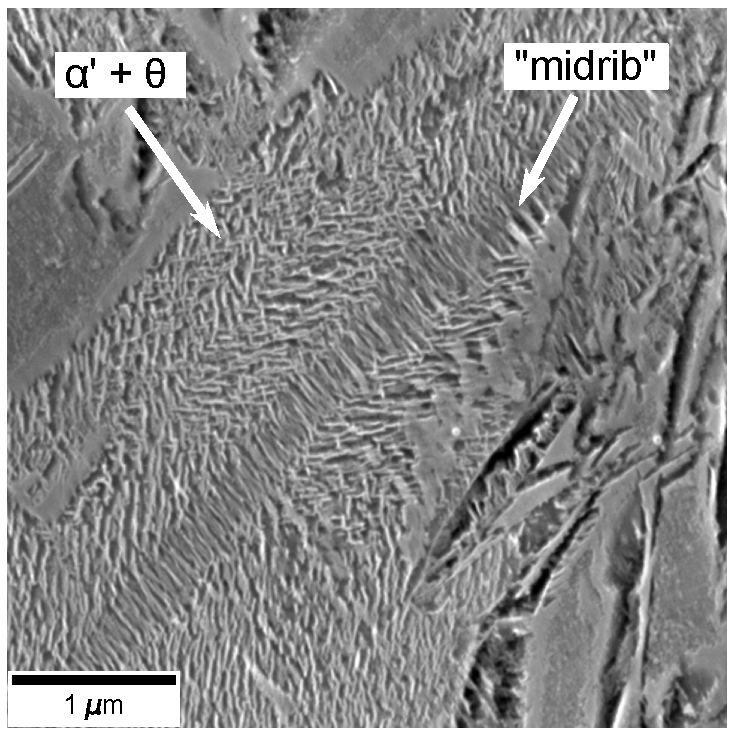
\includegraphics[width=.49\textwidth]{../tese/img/micrografias/170-375/MEV/0/20kx-1.pdf}
  \end{figure}
\end{frame}

\begin{frame}{Microestruturas T\&P}{Efeito do tempo de partição ($t_P$)}
  $T_T = \SI{170}{\degreeCelsius}$; $T_P = \SI{375}{\degreeCelsius}$ / \SI{30}{s}

  \begin{itemize}
      \item EBSD mostra \textbf{\color{green}austenita ($\gamma$) estabilizada}
      \item<2> Bainita não é acompanhada por carbonetos: \textbf{ferrita bainítica ($\alpha_b$)}
      \item<2> $\gamma$ próxima da martensita: evidência de partição!
  \end{itemize}

  \begin{figure}
    \includegraphics<1>[width=.49\textwidth]{../tese/img/micrografias/170-375/MEV/30s/5a.pdf}\hfill
    \includegraphics<1>[width=.49\textwidth]{../tese/img/micrografias/170-375/MEV/30s/5d.pdf}
    
    \includegraphics<2>[width=.49\textwidth]{../tese/img/micrografias/170-375/MEV/30s/5b.pdf}\hfill
    \includegraphics<2>[width=.49\textwidth]{../tese/img/micrografias/170-375/MEV/30s/5e.pdf}
  \end{figure}
\end{frame}

% \begin{frame}{Microestruturas T\&P}{Efeito do tempo de partição ($t_P$)}
%   $T_T = \SI{170}{\degreeCelsius}$; $T_P = \SI{375}{\degreeCelsius}$ / \SI{5}{min}
  
%   \begin{itemize}
%     \item $\alpha_b$ aumenta para tempos mais longos de partição
%     \item $\gamma$ fica mais homogeneamente distribuída
%   \end{itemize}

%   \begin{figure}
%     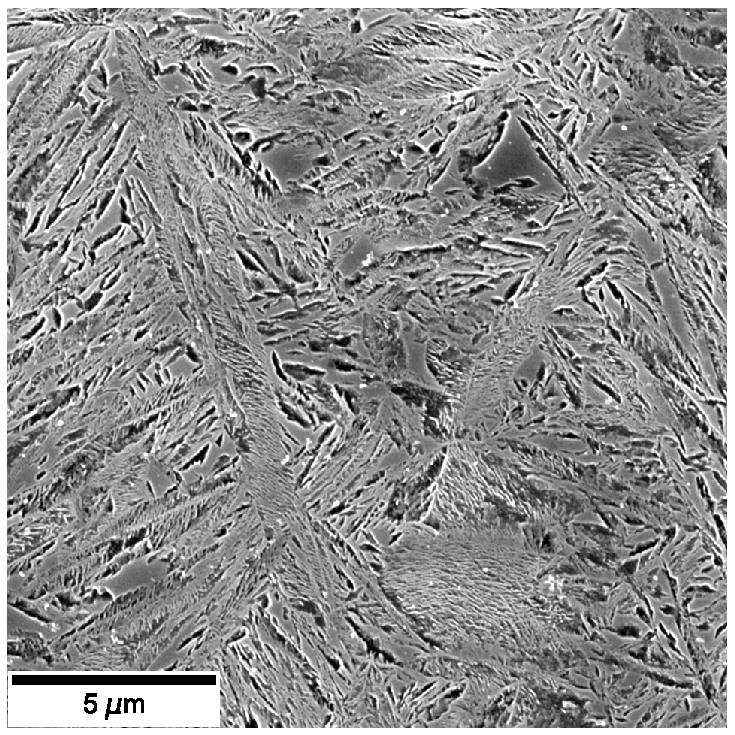
\includegraphics[width=.49\textwidth]{../tese/img/micrografias/170-375/MEV/5min/5kx-6.pdf}\hfill
%     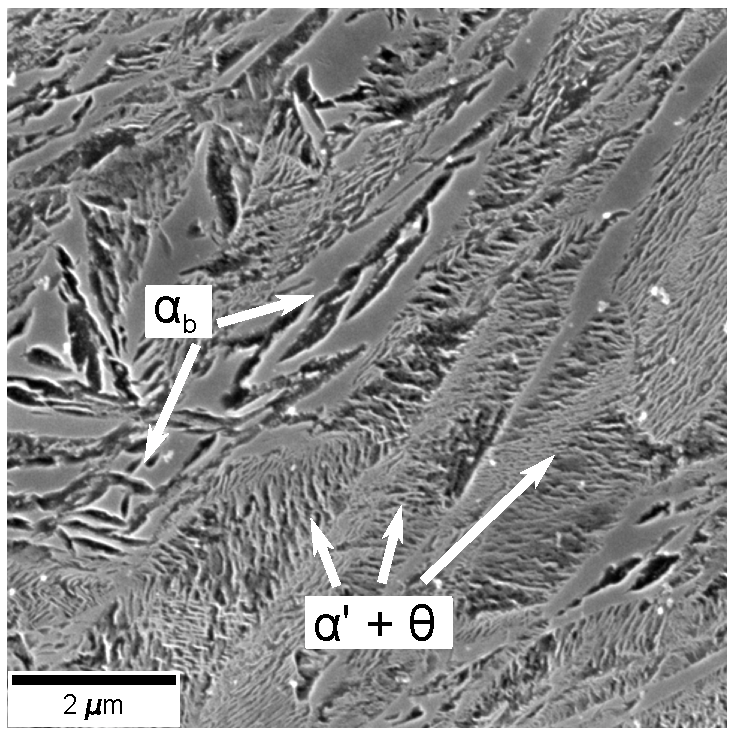
\includegraphics[width=.49\textwidth]{../tese/img/micrografias/170-375/MEV/5min/10kx-4.pdf}
%   \end{figure}
% \end{frame}

\begin{frame}{Microestruturas T\&P}{Efeito do tempo de partição ($t_P$)}
  $T_T = \SI{170}{\degreeCelsius}$; $T_P = \SI{375}{\degreeCelsius}$ / \SI{15}{min}
  
  \begin{figure}
    \includegraphics<1>[width=.49\textwidth]{../tese/img/micrografias/170-375/MEV/15min/1300x.pdf}\hfill
    \includegraphics<1>[width=.49\textwidth]{../tese/img/micrografias/170-375/MEV/15min/QP170-375-15_phase.pdf}
    
    \includegraphics<2>[width=.49\textwidth]{../tese/img/micrografias/170-375/MEV/15min/5kx-8.pdf}\hfill
    \includegraphics<2>[width=.49\textwidth]{../tese/img/micrografias/170-375/MEV/15min/5f.pdf}
  \end{figure}
\end{frame}

\begin{frame}{Microestruturas T\&P}{Efeito do tempo de partição ($t_P$)}
  $T_T = \SI{170}{\degreeCelsius}$; $T_P = \SI{375}{\degreeCelsius}$ / \SI{15}{min}
  
  EPMA
  
  \begin{figure}
    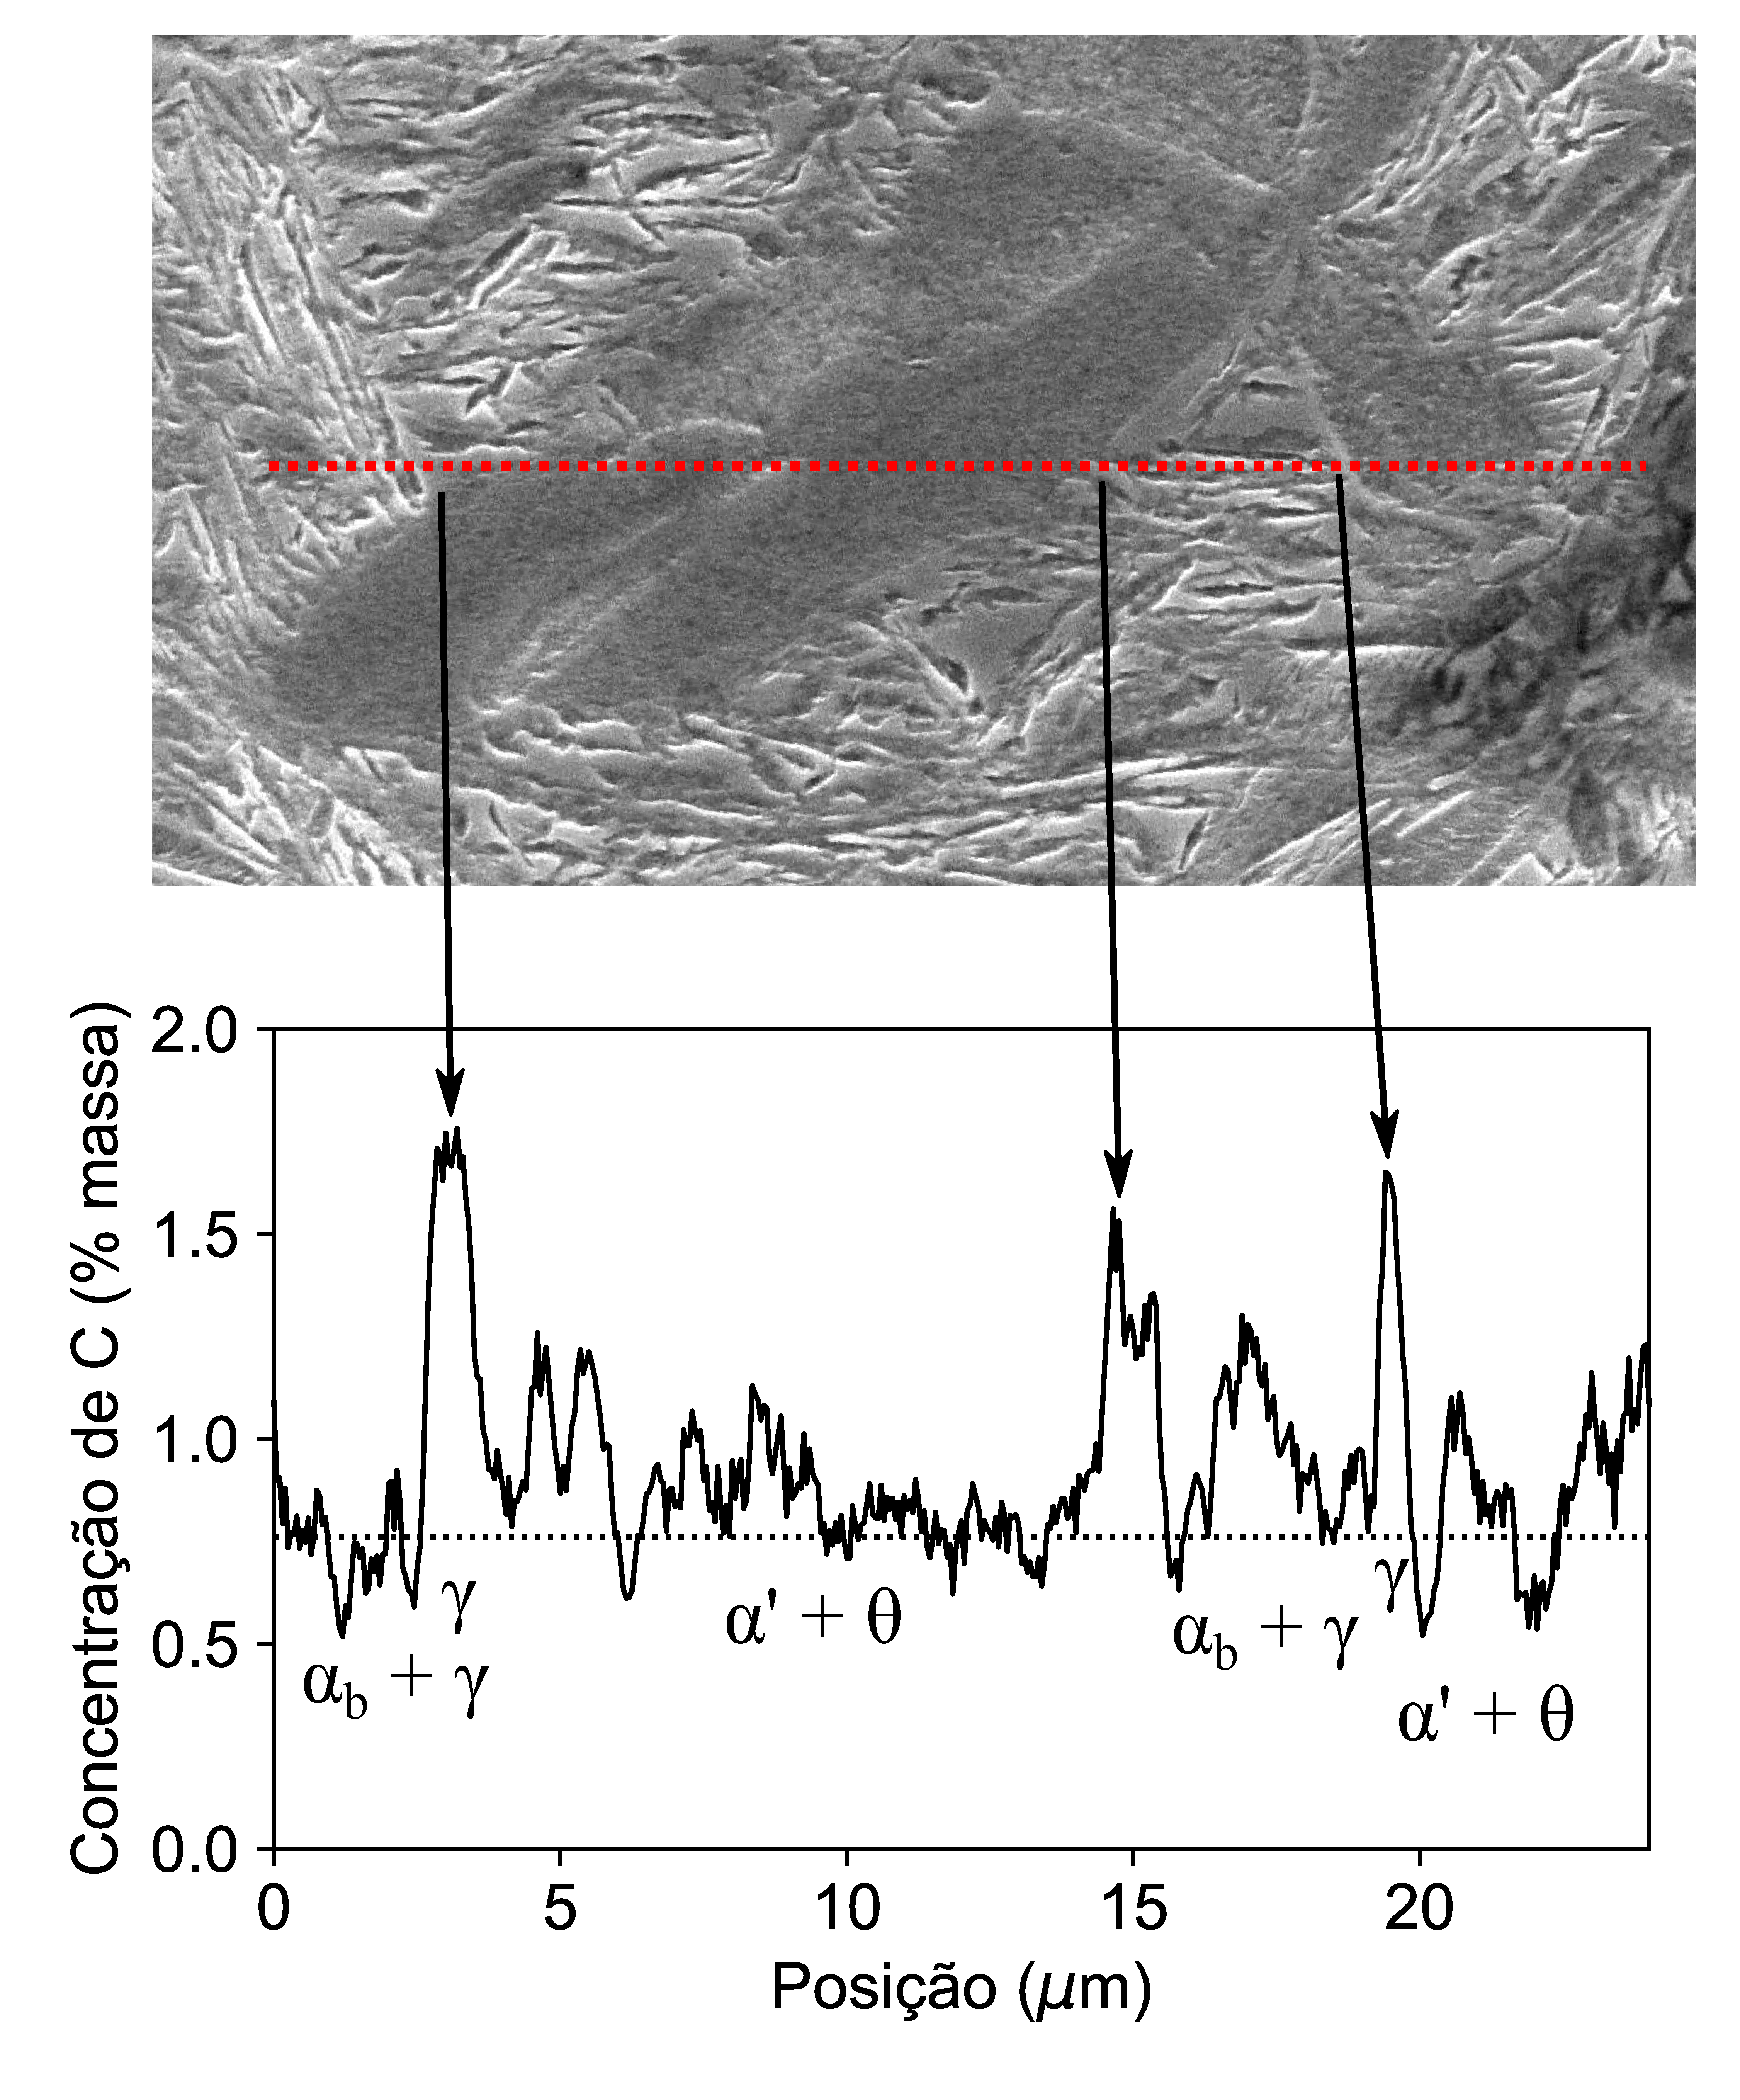
\includegraphics[width=.49\textwidth]{../tese/img/EPMA/0004LIN.pdf}\hfill
    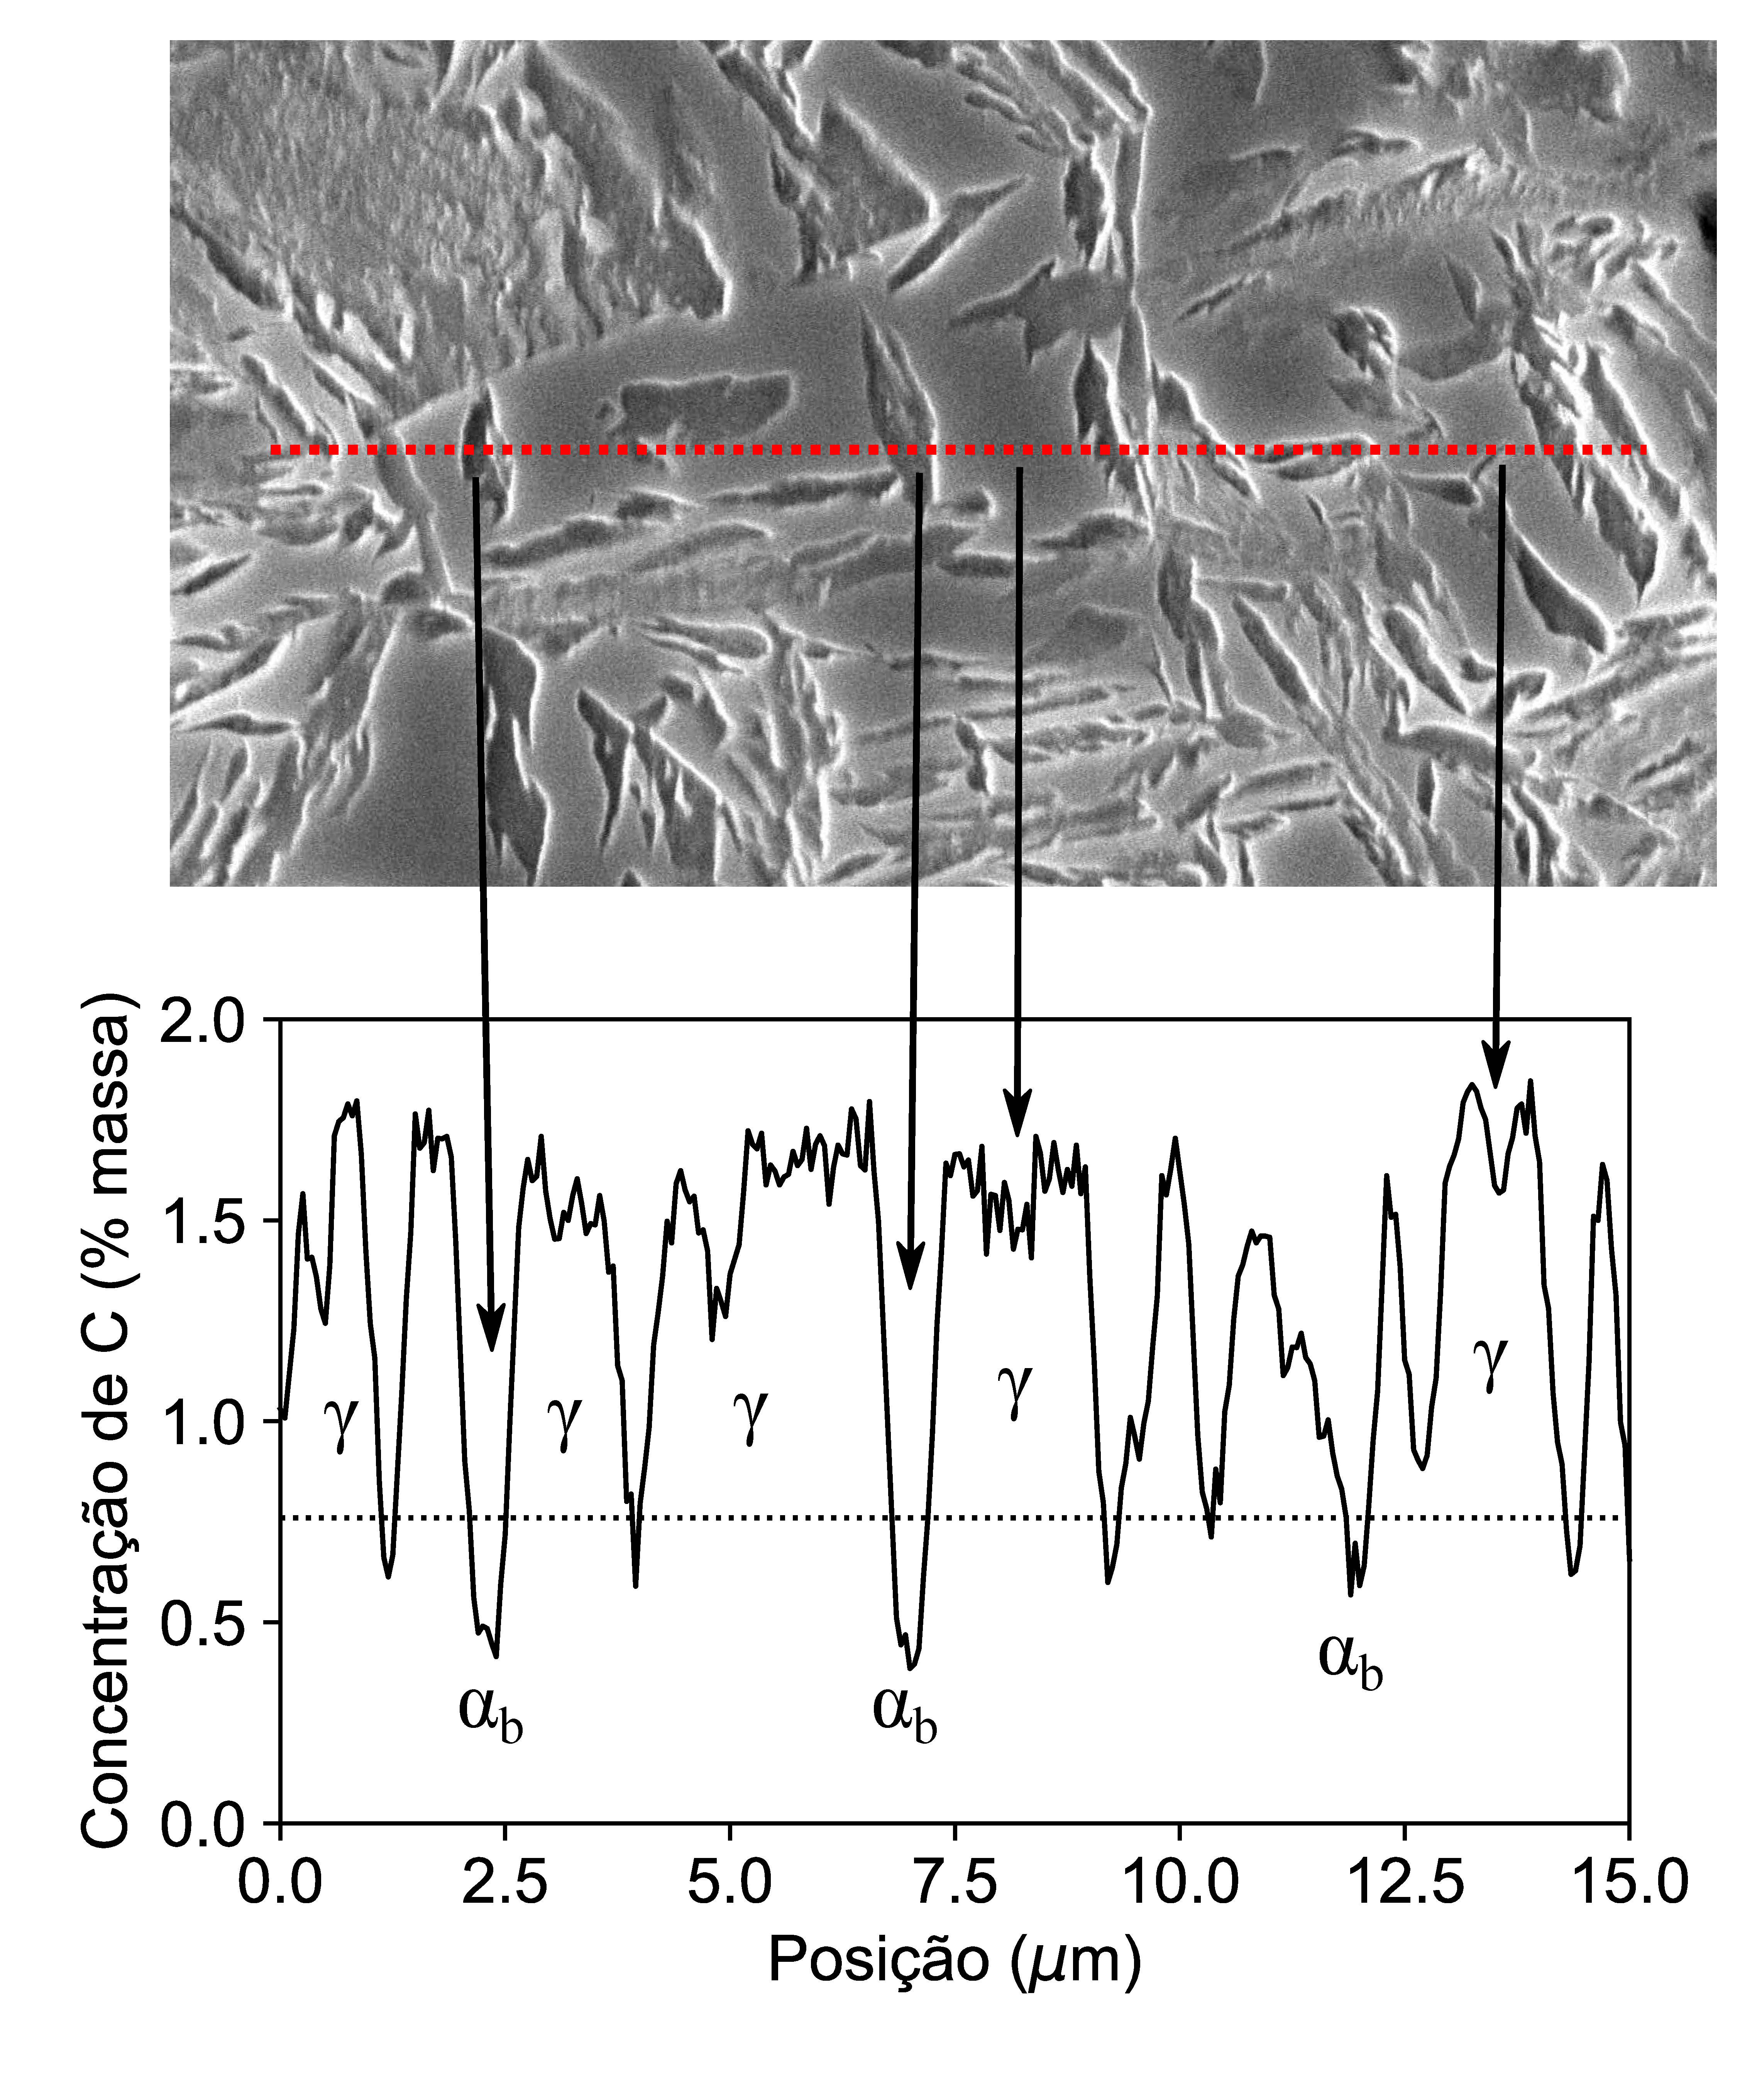
\includegraphics[width=.49\textwidth]{../tese/img/EPMA/0005LIN.pdf}
  \end{figure}
\end{frame}


%%%%%%%%%%%%%%%%%%%%%%%%

\begin{frame}{Microestruturas T\&P}{Efeito da temperatura de partição ($T_P$)}
  $T_T = \SI{170}{\degreeCelsius}$; $T_P = \SI{300}{\degreeCelsius}$ / \SI{15}{min}

  \begin{itemize}
    \item Carbonetos na martensita
    \item $\alpha_b$ mais refinada do que a \SI{375}{\degreeCelsius}
  \end{itemize}

  \begin{figure}
    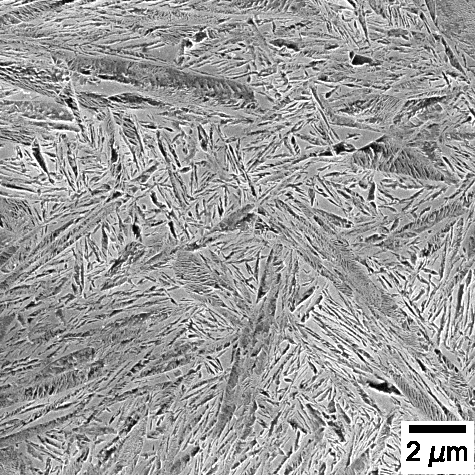
\includegraphics[width=.49\textwidth]{../tese/img/micrografias/170-outros/300C_5kx-3.pdf}\hfill
    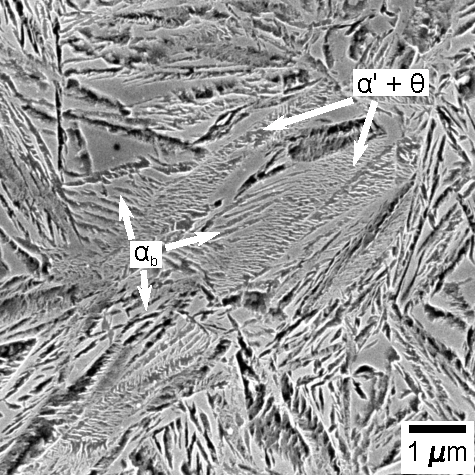
\includegraphics[width=.49\textwidth]{../tese/img/micrografias/170-outros/300C_10kx-1.pdf}
  \end{figure}
\end{frame}

\begin{frame}{Microestruturas T\&P}{Efeito da temperatura de partição ($T_P$)}
  $T_T = \SI{170}{\degreeCelsius}$; $T_P = \SI{450}{\degreeCelsius}$ / \SI{30}{s}

  \begin{itemize}
    \item Carbonetos na martensita
    \item $\alpha_b$ mais grossa do que a \SI{450}{\degreeCelsius}
    \item Nucleação de $\alpha_b$ nos contornos $\alpha' + \theta / \gamma$
  \end{itemize}

  \begin{figure}
    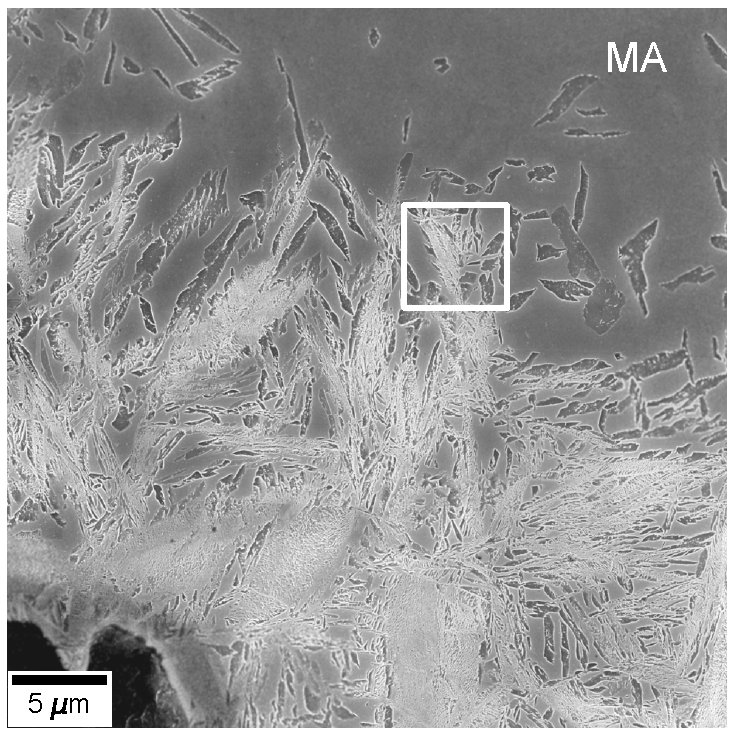
\includegraphics[width=.49\textwidth]{../tese/img/micrografias/170-outros/6b.pdf}\hfill
    % \includegraphics<1>[width=.49\textwidth]{../tese/img/micrografias/170-outros/6c.pdf}\\
    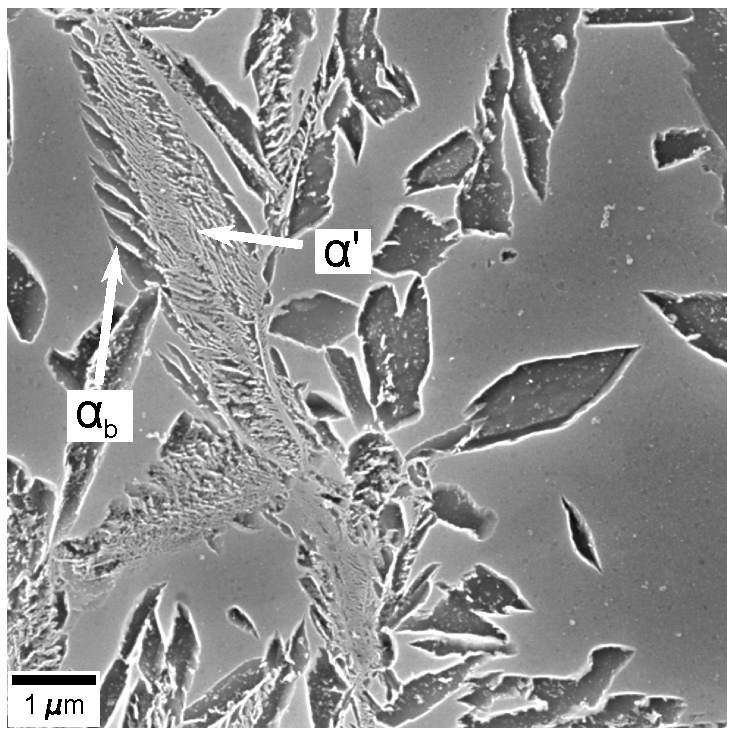
\includegraphics[width=.49\textwidth]{../tese/img/micrografias/170-outros/6d.pdf}
  \end{figure}
\end{frame}

\begin{frame}{Microestruturas T\&P}{Efeito da temperatura de partição ($T_P$)}
  $T_T = \SI{170}{\degreeCelsius}$; $T_P = \SI{450}{\degreeCelsius}$ / \SI{15}{min}

  \begin{itemize}
    \item Toda austenita é consumida após 15~min de partição
  \end{itemize}

  \begin{figure}
    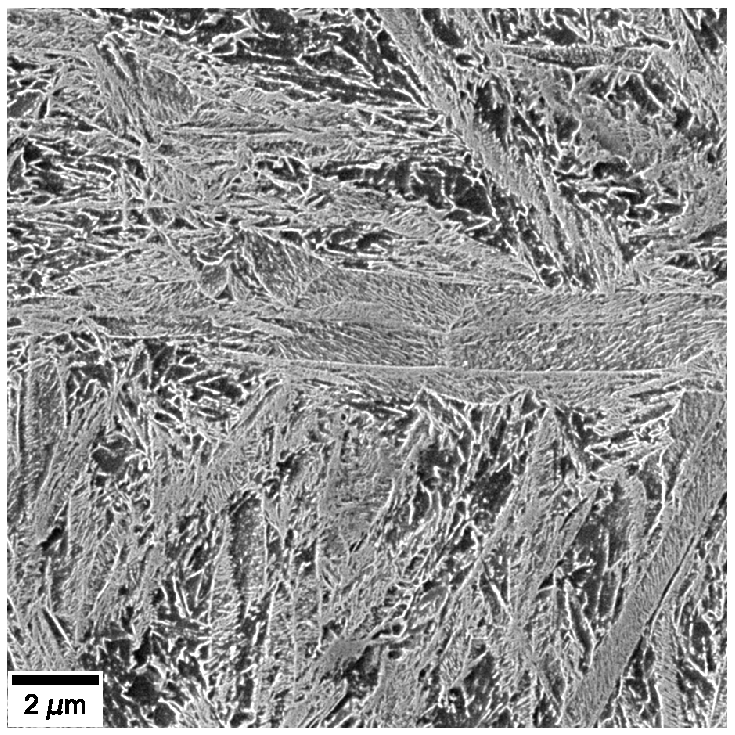
\includegraphics[width=.49\textwidth]{../tese/img/micrografias/170-outros/6e.pdf}\hfill
    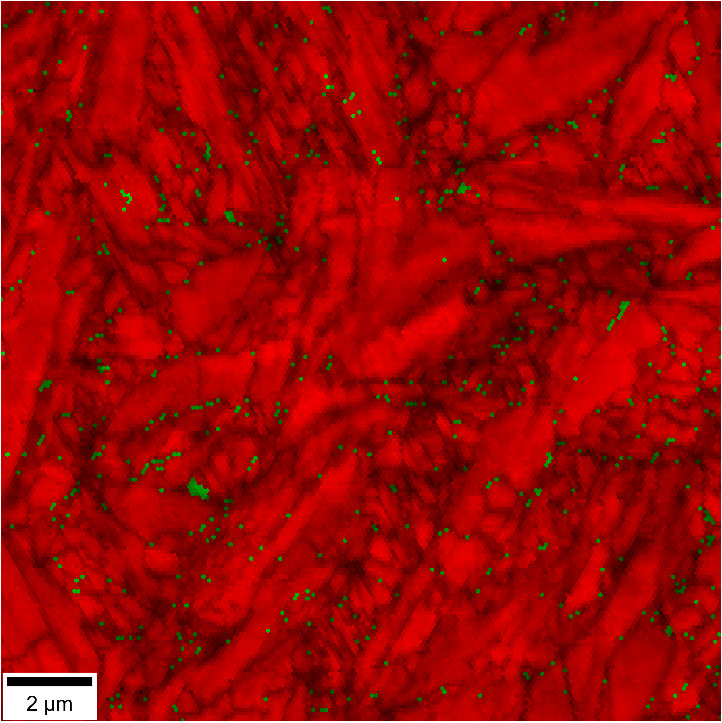
\includegraphics[width=.49\textwidth]{../tese/img/micrografias/170-outros/6f.pdf}
  \end{figure}
\end{frame}


%%%%%%%%%%%%%%%%%%%%%%%%

\begin{frame}{Microestruturas T\&P}{Efeito da temperatura de têmpera ($T_T$)}
  \begin{figure}
    \begin{itemize}
      \item $T_T$ = 140, 170 e \SI{200}{\degreeCelsius}; $T_P$ = \SI{300}{\degreeCelsius}
      \item Bainita é mais refinada quando menor $T_T$ (menores grãos não transformados de austenita)
    \end{itemize}

    \only<1>{\subfloat[$T_T=\SI{140}{\degreeCelsius}$]{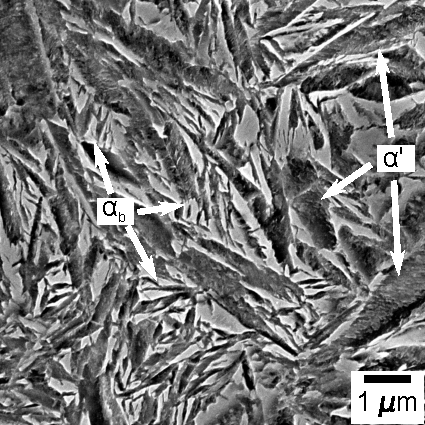
\includegraphics[width=.49\textwidth]{../tese/img/micrografias/efeito_tempera/140-300-2h.pdf}}\hfill}
    \only<1>{\subfloat[$T_T=\SI{170}{\degreeCelsius}$]{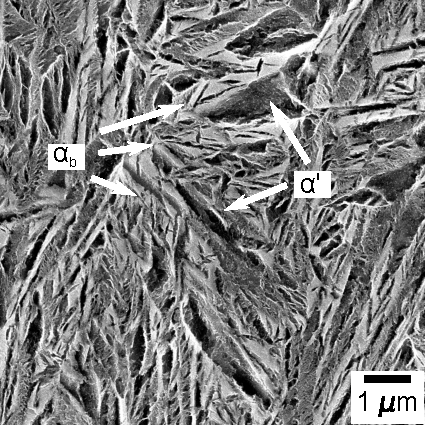
\includegraphics[width=.49\textwidth]{../tese/img/micrografias/efeito_tempera/170-300-2h.pdf}}}
    \only<2>{\subfloat[$T_T=\SI{200}{\degreeCelsius}$]{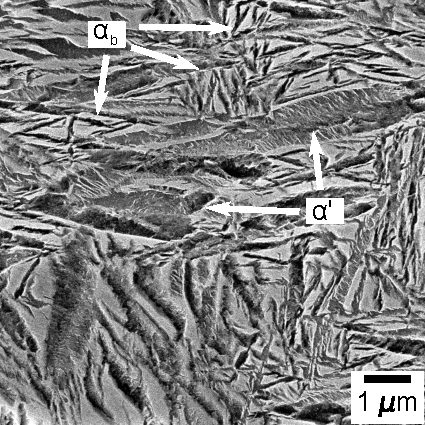
\includegraphics[width=.49\textwidth]{../tese/img/micrografias/efeito_tempera/200-300-2h.pdf}}}
  \end{figure}
\end{frame}

\begin{frame}{Microestruturas T\&P}{Efeito da temperatura de têmpera ($T_T$)}
  \begin{itemize}
    \item Efeito de refinamento da bainita mais claro pela observação da amostra austemperada a \SI{300}{\degreeCelsius}
  \end{itemize}

  \begin{figure}
    \includegraphics[width=.49\textwidth]{../tese/img/micrografias/ADI/300-15min/2500x-1.pdf}\hfill
    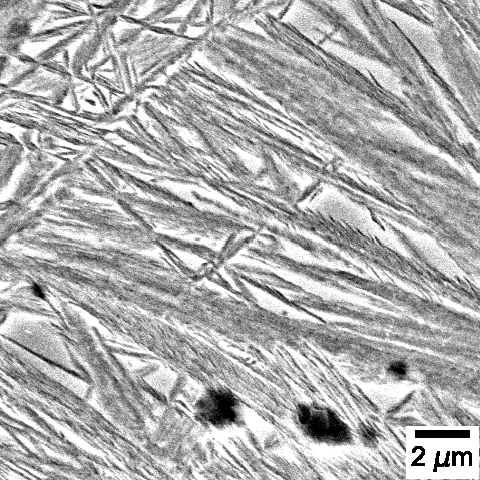
\includegraphics[width=.49\textwidth]{../tese/img/micrografias/ADI/300-15min/10kx-1.pdf}
  \end{figure}
\end{frame}

%%%%%%%%%%%%%%%%%%%%%%%%

\begin{frame}{Microestruturas T\&P}{Carbonetos}
  \begin{itemize}
    \item DRX síncrotron usando detector 2D
    \item $T_T = \SI{170}{\degreeCelsius}$
  \end{itemize}

  \begin{figure}
    \includegraphics<1>[width=\textwidth]{img/selected_diffractograms.pdf}
    \includegraphics<2>[width=\textwidth]{img/selected_diffractograms_detail.pdf}
  \end{figure}  
\end{frame}

\begin{frame}{Microestruturas T\&P}{Carbonetos}
  \begin{itemize}
    \item Cementita a \SI{450}{\degreeCelsius}
  \end{itemize}  

  \begin{figure}
    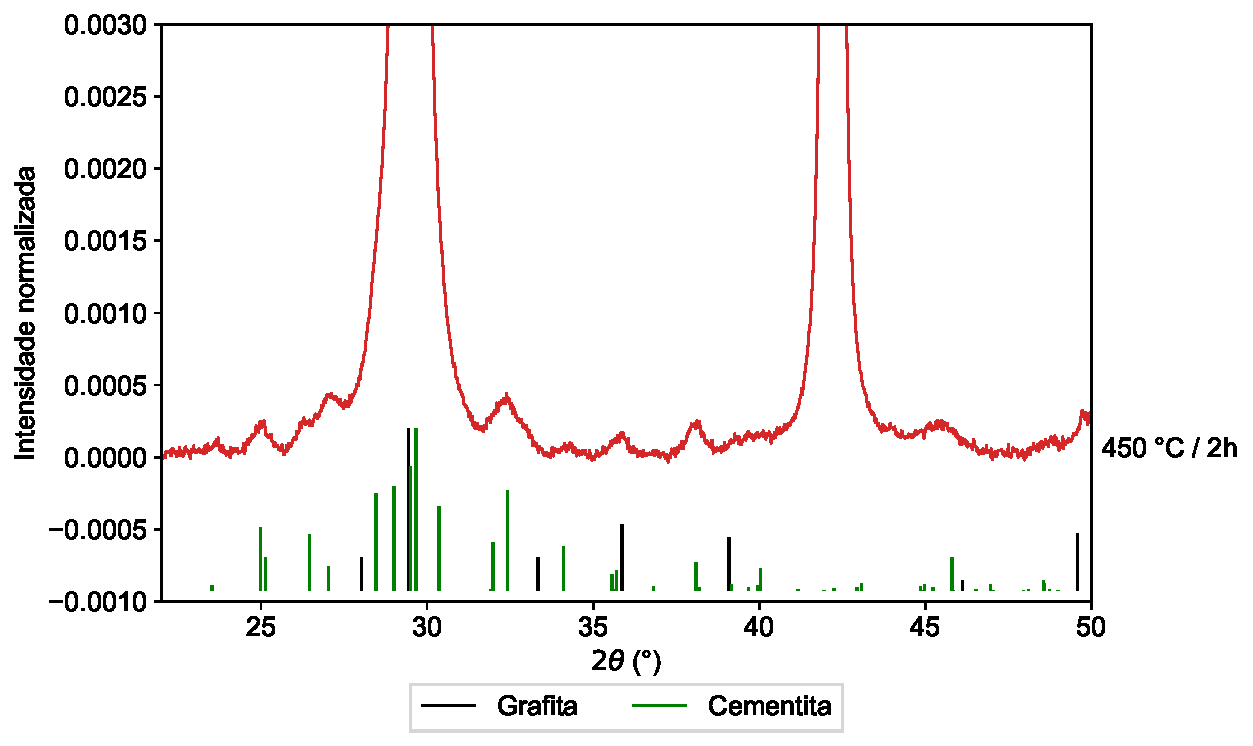
\includegraphics[width=\textwidth]{img/selected_diffractograms_cementite.pdf}
  \end{figure}
\end{frame}

\begin{frame}{Microestruturas T\&P}{Carbonetos}
  \begin{itemize}
    \item Carbonetos $\epsilon$ ou $\eta$ a 300 e \SI{375}{\degreeCelsius}
  \end{itemize}  

  \begin{figure}
    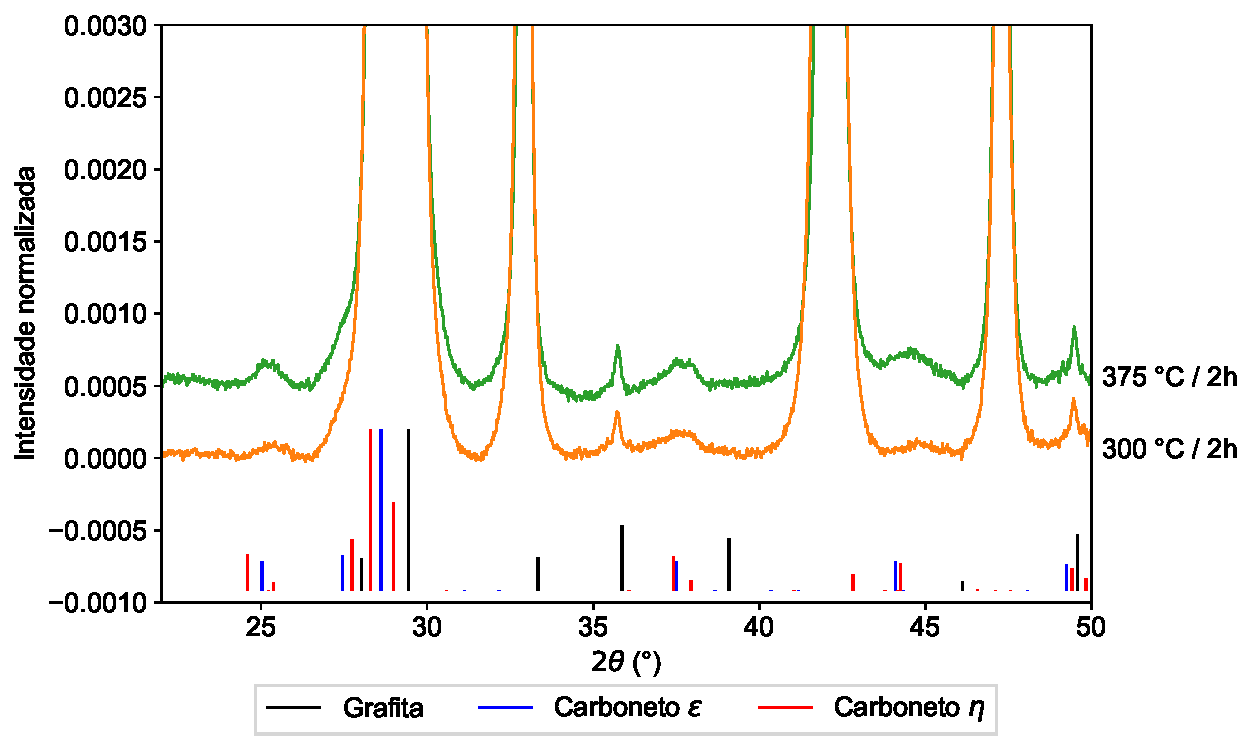
\includegraphics[width=.93\textwidth]{img/selected_diffractograms_eta.pdf}
  \end{figure}
\end{frame}

%%%%%%%%%%%%%%%%%%%%%%%%%%%%

\subsection{Cinética das transformações de fases durante T\&P}

\begin{frame}{Cinética}{Dilatometria}
  \begin{itemize}
    \item $T_T = \SI{170}{\degreeCelsius}$
    \item Dilatação durante a etapa de partição: expansão em todas as condições
    \item Contração a \SI{450}{\degreeCelsius}: cementita
  \end{itemize}

  \begin{figure}
    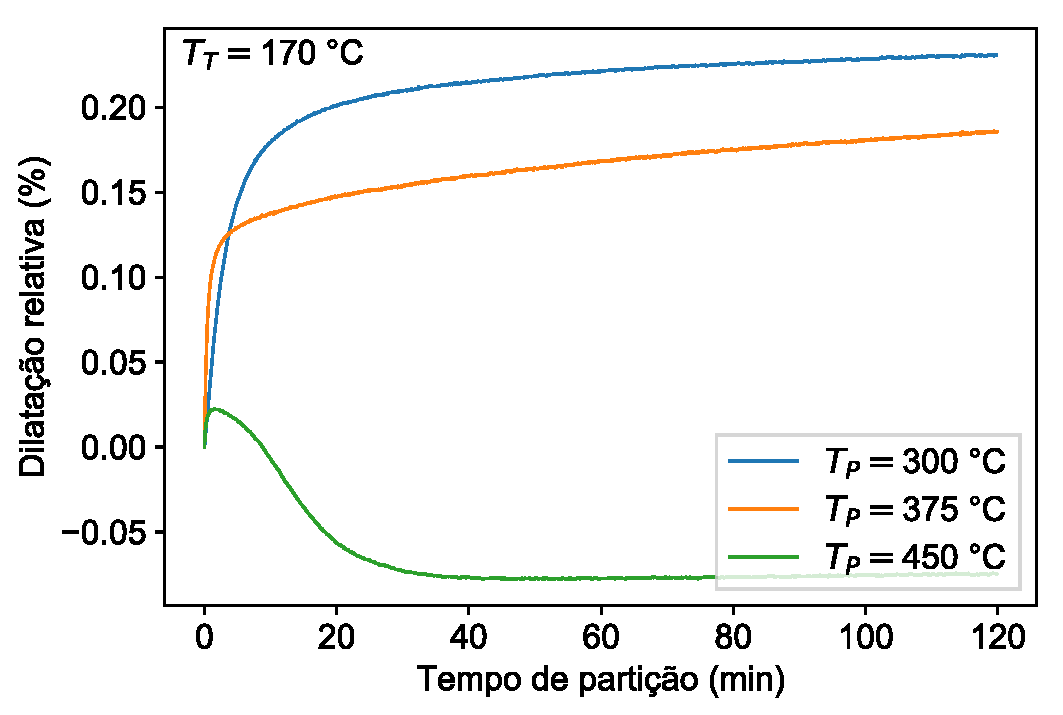
\includegraphics[width=.8\textwidth]{../tese/img/dilatometria/dlxt_QT=170-PT.pdf}
    % \includegraphics<2>[width=.8\textwidth]{../tese/img/dilatometria/dil_extra.pdf}
  \end{figure}
\end{frame}

\begin{frame}{Cinética}{Dilatometria}
  \begin{itemize}
    \item Austêmpera (sem martensita): expansão ocorre mais lentamente; tempo de incubação
    \item<2> $T_P = \SI{300}{\degreeCelsius}$, variando $T_T$
  \end{itemize}

  \begin{figure}
    \includegraphics<1>[width=.8\textwidth]{../tese/img/dilatometria/dlxt_austempera.pdf}
    \includegraphics<2>[width=.8\textwidth]{../tese/img/dilatometria/dlxt_PT300.pdf}
  \end{figure}
\end{frame}

\begin{frame}{Cinética}{Dilatometria}
  \begin{itemize}
    \item Presença da martensita afeta a cinética da reação bainítica
    \item Como mostra micrografias, nucleação de $\alpha_b$ ocorre nas interfaces $\alpha'/\theta$
  \end{itemize}
\end{frame}

% \begin{frame}{Cinética}{Dilatometria}
%   \begin{itemize}
%     \item $T_T = \SI{170}{\degreeCelsius}$
%     \item Dilatação $\times$ temperatura
%     \item<1> $t_P = 2~h$: Desvio da dilatação esperada $\rightarrow$ reação bainítica começa antes de $T_P$ ser atingido
%     \item<2> $t_P = 30~s$: Formação de $\alpha'_{fr}$ no resfriamento final
%   \end{itemize}

%   \begin{figure}
%     \includegraphics<1>[width=.8\textwidth]{../tese/img/dilatometria/dlxT_qPT2h_fc.pdf}
%     \includegraphics<2>[width=.8\textwidth]{../tese/img/dilatometria/dlxT_qPT30s-fc.pdf}
%   \end{figure}
% \end{frame}

%%%%%%%%%%%%%%%%%%%%%%%%%%%%%%%%%% DRX in situ

\begin{frame}{Cinética}{Difração de raios X \textit{in situ}}
  \begin{itemize}
    % \item $T_T = \SI{170}{\degreeCelsius}$; $T_P = \SI{300}{\degreeCelsius} / 2~h$; 
    % \item Eixo X: $2\theta$; eixo Y: Tempo de partição [s]
    \item Evolução do pico (111)$\gamma$: atenuação e deslocamento para maiores valores de distância interplanar $\rightarrow$ Reação bainítica consome $\gamma$; carbono distorce $\gamma$
  \end{itemize}

  \begin{figure}
    \includegraphics[width=.8\textwidth]<1>{../tese/img/XTMS/XTMS_colormap_full.pdf}
    \includegraphics[width=.8\textwidth]<2>{../tese/img/XTMS/XTMS_colormap_detail.pdf}
  \end{figure}
\end{frame}

\begin{frame}{Cinética}{Difração de raios X \textit{in situ}}
  \begin{itemize}
    \item $T_T = \SI{170}{\degreeCelsius}$
    \item Fração de ferrita bainítica $f^{\alpha_b}$ calculada assumindo que $f^{\alpha'}$ é constante
    \item A \SI{450}{\degreeCelsius} toda $\gamma$ é consumida
    \item<2> $f^{\alpha_b}$ para $t_P = 0$ é maior do que zero $\rightarrow$ $\alpha_b$ no aquecimento
  \end{itemize}

  \begin{figure}
    \includegraphics<1>[width=.85\textwidth]{../tese/img/XTMS/XTMS_ph_fraction.pdf}
    \includegraphics<2>[width=.85\textwidth]{../tese/img/XTMS/XTMS_ph_fraction_detail.pdf}
  \end{figure}
\end{frame}

\begin{frame}{Cinética}{Difração de raios X \textit{in situ}}
  \begin{itemize}
    \item Em todas condições $\gamma$ enriquece em carbono
    \item Tendências parecem com as curvas de $f^{\alpha_b}$
    \item Sugere que enriquecimento em C de $\gamma$ é controlado por formação de $\alpha_b$
  \end{itemize}

  \begin{figure}
    \centering
    \includegraphics<1>[width=.8\textwidth]{../tese/img/XTMS/XTMS_wC.pdf}
    \includegraphics<2>[width=.8\textwidth]{../tese/img/XTMS/XTMS_wC_detail.pdf}
  \end{figure}
\end{frame}

\begin{frame}
  \begin{itemize}
    \item Limite termodinâmico da partição de carbono
    \item Toji, Miyamoto e Raabe (2015)\footnotemark[1] observaram experimentalmente a partição de carbono entre $(\alpha' + \theta)$ e $\gamma$ mesmo na presença de $\theta$ precipitado em $\alpha'$
    \item<2> Partição de carbono é possível se $\mu_C^{\alpha' + \theta} > \mu_C^\gamma$
    \item<2> Modelo ECC$\theta$ (CCE$\theta$) de Toji: carbono em $\gamma$ ($w_C^\gamma$) após partição na presença de $\theta$
    \item<2> $w_C^\gamma$ depende da energia livre de $\theta$, mas não de $f^{\alpha'}$
  \end{itemize}

  \begin{figure}
    \includegraphics<1>[width=\textwidth]{img/toji_2015.pdf}
    \includegraphics<2>[width=.7\textwidth]{../tese/img/common_tangent.pdf}
  \end{figure}

  \footnotetext[1]{Toji, Y., Miyamoto, G. \& Raabe, D. Carbon partitioning during quenching and partitioning heat treatment accompanied by carbide precipitation. Acta Mater. 86, 137–147 (2015).}
\end{frame}

\begin{frame}
  \begin{itemize}
    \item ECC$\theta$ na liga estudada para diferentes carbonetos
    \item Extremos: ortocementita (mais estável, partição de elementos substitucionais) e paracementita (cementita de paraequilíbrio)
  \end{itemize}

  \begin{figure}
    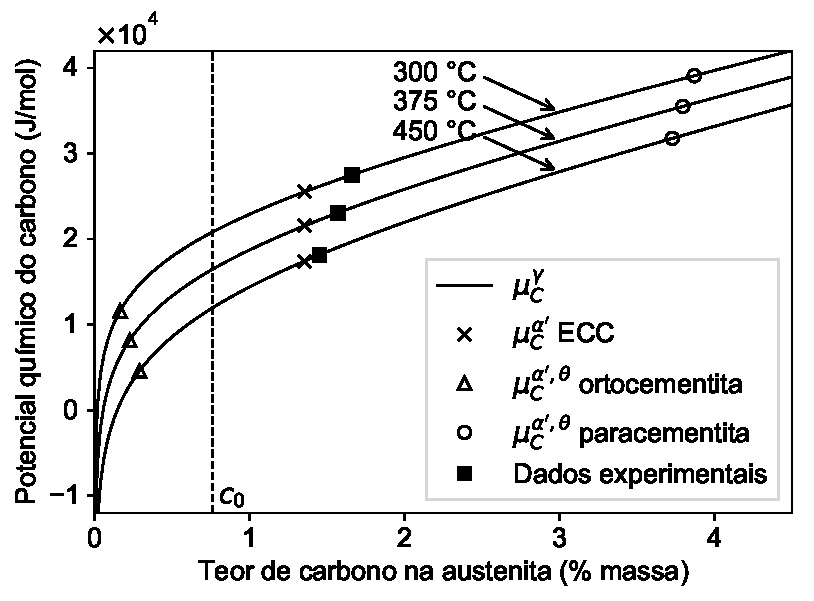
\includegraphics[width=.8\textwidth]{../tese/img/thermo-calc/CCE.pdf}
  \end{figure}
\end{frame}

\begin{frame}
  \begin{itemize}
    \item Limite termodinâmico da reação bainítica
    \item Pela teoria difusional: paraequilíbrio; pela teoria sem difusão: $T_0$ ou $T_0'$
    \item Paraequilíbrio não descreve bem resultados experimentais
    \item Modelo WBs Hillert\footnotemark[1]: força motriz adicional calculada a partir de dados empíricos
  \end{itemize}

  \begin{figure}
    \includegraphics[width=.8\textwidth]{../tese/img/thermo-calc/WBs_para.pdf}
  \end{figure}

  \footnotetext[1]{Hillert, M., Höglund, L. \& Ågren, J. Escape of carbon from ferrite plates in austenite. Acta Metall. Mater. 41, 1951–1957 (1993).}
\end{frame}


\begin{frame}{Resumo dos resultados experimentais}
  \begin{itemize}
    \item Segregação causa distribuição heterogênea de $\alpha'$: regiões próximas de contornos de célula apresentam menos $\alpha'$
    \item Carbonetos precipitam em $\alpha'$ durante o aquecimento de $T_T$ a $T_P$
    \item Partição de carbono entre $\alpha + \theta$ e $\gamma$ acontece para curtos tempos
    \item Carbonetos não são completamente dissolvidos durante partição
    \item Reação bainítica acontece durante a etapa de partição
    \item Curvas de $f^{\alpha_b}$ e $w_C^\gamma$ e modelo WBs sugerem que enriquecimento em C de $\gamma$ é controlado por formação de $\alpha_b$
  \end{itemize}
\end{frame}


%%%%%%%%%%%%%%%%%%%%%%%%%%%%%%


\subsection{Modelo computacional de redistribuição de carbono}

\begin{frame}{Modelo redistribuição de C}
  Hipótese: poderia o \textit{soft impingement} (interação dos perfis de difusão) desacelerar a partição de carbono entre $\alpha'$ ($\alpha' + \theta$) e $\gamma$?

  \begin{figure}
    \includegraphics[width=.8\textwidth]{img/C_profiles.pdf}
  \end{figure}

  Simulações computacionais: crescimento $\alpha_b$ e partição de carbono entre $\alpha' + \theta$ e $\gamma$
\end{frame}

\begin{frame}{Modelo redistribuição de C}{Metodologia}
  % Na literatura: Mujahid e Bhadeshia, 1992; Hillert et al, 1992; Santofimia et al., 2008, 2009: partição de carbono entre placa supersaturada em carbono de ferrita e austenita
  % It consists of a mixed-model assuming both Zener's theory of diffusional transformations and Christian's theory of interface controlled phase transformations

  \begin{itemize}
    \item Apenas partição de carbono (paraequilíbrio)

    \item Igualdade dos potenciais químicos de C na interface

    \item Fluxos de carbono são balanceados pelo problema de Stefan:
    
    $$-D_C^\alpha \frac{d c^\alpha}{d z}\Bigg|_{int} + v\left(c^\gamma_{int} - c^\alpha_{int} \right) = -D_C^\gamma \frac{d c^\gamma}{d z}\Bigg|_{int}$$

    \item Interfaces $(\alpha' + \theta)/\gamma$ são fixas ($v = 0$)

    \item Interfaces $\alpha_b/\gamma$ são móveis. Velocidade é contabilizada pelo modelo de modo misto ($v = \frac{M}{V_m} \Delta G_{quim}$)

    \item Dados termodinâmicos (potenciais químicos) obtidos usando Thermo-Calc (TCFE8)

    \item Segunda lei de Fick resolvida numericamente utilizando o método de diferenças finitas
    
    $$ \frac{\partial c}{\partial t} = \frac{\partial}{\partial z} \left( D \frac{\partial c}{\partial z} \right) $$
  \end{itemize}
\end{frame}

\begin{frame}{Modelo redistribuição de C}
  Resultados divididos em duas partes:

  \begin{itemize}
    \item Sem bainita + efeito da precipitação de carbonetos com diferentes energias livres
    \item Com bainita + efeito da precipitação de carbonetos com diferentes energias livres
  \end{itemize}
\end{frame}

\begin{frame}{Partição de carbono $(\alpha' + \theta)/\gamma$}
  \begin{itemize}
    \item Simulações sem bainita
    \item Quando considerados, carbonetos estão presentes desde $t_P = 0$
    \item Composição interfacial em $\gamma$ determinado pelo modelo ECC$\theta$
    \item Geometria equivalente a T\&P com $T_T = \SI{170}{\degreeCelsius}$ ($f^{\alpha'} = 43\%$) e $T_P = \SI{375}{\degreeCelsius}$
    \item Largura das regiões das fases: $\alpha'$ \SI{1.0}{\mu m}; $\gamma$ \SI{1.32}{\mu m}
  \end{itemize}

  \begin{figure}
    \includegraphics[width=.8\textwidth]{img/simulations_nobainite.pdf}
  \end{figure}
\end{frame}

\begin{frame}{Partição de carbono $\alpha'/\gamma$}
  Sem carbonetos

  \begin{itemize}
    \item Caso mais simples de todos
    \item C em $\gamma$ na interface cresce rapidamente (max. $\approx$~4,5\%)
    \item Partição muito rápida: todo C em $\alpha'$ difunde para austenita em cerca de 1~s
  \end{itemize}

  \begin{figure}
    \includegraphics[width=.55\textwidth]{../tese/img/cpartition/cprofiles/mart_FoFo_CCE.pdf}
  \end{figure}
\end{frame}

\begin{frame}{Partição de carbono $(\alpha' + \theta)/\gamma$}
  $\theta$: Ortocementita

  \begin{itemize}
    \item $\mu_C^{\alpha' + \theta} < \mu_C^\gamma \rightarrow$ Carbono interfacial em $\gamma$ calculado pelo ECC$\theta$ é \emph{menor do que $c_0$}
    \item Difusão de carbono acontece de $\gamma$ para $\alpha' + \theta$
    \item \emph{Aumento de carbono em $\alpha' + \theta \rightarrow$ aumento da fração de carbonetos}
  \end{itemize}

  \begin{figure}
    \includegraphics<1>[width=.55\textwidth]{../tese/img/cpartition/cprofiles/mart_FoFo_CCEortho.pdf}
    % \includegraphics<2>[width=.55\textwidth]{../tese/img/cpartition/muprofiles/mart_FoFo_CCEortho.pdf}
  \end{figure}
\end{frame}

\begin{frame}{Partição de carbono $(\alpha' + \theta)/\gamma$}
  $\theta$: Paracementita

  \begin{itemize}
    \item Paracementita: carboneto de alta energia livre (interação negativa Si-C aumenta atividade de C)
    \item $\mu_C^{\alpha' + \theta} > \mu_C^\gamma \rightarrow$ partição ocorre de $\alpha' + \theta$ para $\gamma$
    \item \emph{Diminuição de carbono em $\alpha' + \theta \rightarrow$ diminuição da fração de carbonetos}
    \item Partição é mais lenta do que no cenário sem carbonetos
  \end{itemize}

  \begin{figure}
    \includegraphics<1>[width=.55\textwidth]{../tese/img/cpartition/cprofiles/mart_FoFo_CCEpara.pdf}
    % \includegraphics<2>[width=.55\textwidth]{../tese/img/cpartition/muprofiles/mart_FoFo_CCEpara.pdf}
  \end{figure}
\end{frame}

\begin{frame}{Partição de carbono $(\alpha' + \theta)/\gamma$}
  \begin{itemize}
    \item Nem ortocementita nem paracementita devem representar bem carbonetos de transição
    \item Dados termodinâmicos de carbonetos de transição não são encontrados na literatura
    \item Simulações feitas para carbonetos com energias livres variando de ortocementita para paracementita
  \end{itemize}

  \begin{figure}
    \includegraphics[width=.7\textwidth]{../tese/img/thermo-calc/CCE.pdf}
  \end{figure}
\end{frame}

\begin{frame}{Partição de carbono $(\alpha' + \theta)/\gamma$}
    \begin{itemize}
      \item Energias livres representadas pelo potencial químico $\mu_C^{\alpha' + \theta}$
      \item Partição é mais lenta quando os carbonetos possuem menor energia livre (mais estáveis)
      \item $\theta$ mais estável $\rightarrow$ menor carbono interfacial em $\gamma$ $\rightarrow$ difusão de C mais lenta
    \end{itemize}

  \begin{figure}
    \includegraphics[width=.8\textwidth]{../tese/img/cpartition/nobainite_cavg.pdf}
  \end{figure}
\end{frame}

%%%%%%% Com bainita

\begin{frame}{Partição de carbono $(\alpha' + \theta)/\gamma$ + crescimento de $\alpha_b$}
  \begin{itemize}
    \item Simulações com bainita
    \item Potenciais químicos de C em $\alpha_b$ modificados de acordo com o modelo WBs de Hillert
    \item Nucleação de $\alpha_b$ a $t_P = 0$ (sem tempo de incubação)
    % \item Quando considerados, carbonetos estão presentes desde $t_P = 0$
    % \item Composição interfacial em $\gamma$ determinado pelo modelo ECC$\theta$
    % \item Geometria equivalente a T\&P com $T_T = \SI{170}{\degreeCelsius}$ ($f^{\alpha'} = 43\%$) e $T_P = \SI{375}{\degreeCelsius}$
    % \item Largura das regiões das fases: $\alpha'$ \SI{1.0}{\mu m}; $\gamma$ \SI{1.32}{\mu m}
  \end{itemize}

  \begin{figure}
    \includegraphics[width=.8\textwidth]{img/simulations_bainite.pdf}
  \end{figure}
\end{frame}

\begin{frame}{Partição de carbono $(\alpha' + \theta)/\gamma$ + crescimento de $\alpha_b$}
  Sem carbonetos
  \begin{figure}
    \href[pdfnewwindow]{animacoes/coupled_FoFo_375_CCE.mp4}{
      \includegraphics[width=.7\textwidth]{../tese/img/cpartition/cprofiles/coupled_FoFo_375_CCE_sep.pdf}
    }
    % \includegraphics<2>[width=\textwidth]{../tese/img/cpartition/muprofiles/coupled_FoFo_375_CCE.pdf}
  \end{figure}
\end{frame}

\begin{frame}{Partição de carbono $(\alpha' + \theta)/\gamma$ + crescimento de $\alpha_b$}
  \begin{itemize}
    \item Força motriz para crescimento de $\alpha_b$ descresce até eventualmente ficar negativa $\rightarrow$ sentido de movimentação da interface é invertido
  \end{itemize}

  \begin{figure}
    \includegraphics[height=.65\textwidth]{../tese/img/cpartition/aus1fer1_interface_DF.pdf}
    % \includegraphics<2>[height=.65\textwidth]{../tese/img/cpartition/aus1fer1_interface_comp.pdf}
  \end{figure}
\end{frame}

\begin{frame}{Partição de carbono $(\alpha' + \theta)/\gamma$ + crescimento de $\alpha_b$}
  Ortocementita
  \begin{figure}
    \href[pdfnewwindow]{animacoes/coupled_FoFo_375_CCEortho.mp4}{
      \includegraphics[width=.7\textwidth]{../tese/img/cpartition/cprofiles/coupled_FoFo_375_CCEortho_sep.pdf}
    }
  \end{figure}
\end{frame}

\begin{frame}{Partição de carbono $(\alpha' + \theta)/\gamma$ + crescimento de $\alpha_b$}
  Paracementita
  \begin{figure}
    \href[pdfnewwindow]{animacoes/coupled_FoFo_375_CCEpara.mp4}{
      \includegraphics[width=.7\textwidth]{../tese/img/cpartition/cprofiles/coupled_FoFo_375_CCEpara_sep.pdf}
    }
  \end{figure}
\end{frame}

\begin{frame}{Partição de C $(\alpha' + \theta)/\gamma$ + crescimento de $\alpha_b$}
  $\mu_C = \SI{23.2}{kJ/mol} \rightarrow$ composição de $\gamma$ na interface $(\alpha' + \theta)/\gamma$ = WBs
  \begin{figure}
    \href[pdfnewwindow]{animacoes/coupled_FoFo_375_mu23e3.mp4}{
      \includegraphics[width=.7\textwidth]{../tese/img/cpartition/cprofiles/coupled_FoFo_375_mu23e3_sep.pdf}
    }
  \end{figure}
\end{frame}

\begin{frame}
  \begin{itemize}
    \item $\mu_C = \SI{23.2}{kJ/mol} \rightarrow$ \textit{soft impingement} faz que a partição de C entre $\alpha' + \theta$ e $\gamma$ cesse
    \item $\mu_C > \SI{23.2}{kJ/mol} \rightarrow$ partição de C ocorre de $\alpha' + \theta$ para $\gamma$ para curtos tempos. Para tempos suficientemente longos a direção é invertida
    \item<2> Comparação quando não há bainita
  \end{itemize}

  \begin{figure}
    \includegraphics<1>[width=.7\textwidth]{../tese/img/cpartition/coupled_cavg.pdf}
    \includegraphics<2>[width=.7\textwidth]{../tese/img/cpartition/all_cavg.pdf}
  \end{figure}
\end{frame}

\begin{frame}
  \begin{figure}
    \includegraphics[width=\textwidth]{../tese/img/cpartition/coupled_cavg_mu20e3.pdf}
  \end{figure}
\end{frame}

% \begin{frame}
%   \begin{figure}
%     \includegraphics[width=\textwidth]{../tese/img/banana_plot-pt.pdf}
%   \end{figure}
% \end{frame}


\section{Conclusões}

\begin{frame}{Conclusões}
  % O presente trabalho procurou estudar aspectos de transformações de fases --- com ênfase na evolução microestrutural e cinética das reações --- do tratamento térmico de Têmpera e Partição (T\&P) aplicado a uma liga de ferro fundido nodular. Em relação às observações experimentais, as seguintes conclusões foram obtidas:

  \begin{enumerate}
    \item \textbf{Microssegregação} não foi completamente eliminada durante a austenitização e causa uma \textbf{distribuição heterogênea da martensita}. Contornos de célula apresentam mais martensita do que regiões próximas a nódulos de grafita.

    \item Precipitação de \textbf{carbonetos na martensita} acontece durante o aquecimento desde a temperatura de têmpera até a temperatura de partição. Carbonetos de transição ($\eta$ ou $\epsilon$) são precipitados a 300 e a \SI{375}{\degreeCelsius}. Cementita precipita a \SI{450}{\degreeCelsius}.

    \item A \textbf{reação bainítica} acontece durante a etapa de partição. Para $T_P$ igual a 300 e \SI{375}{\degreeCelsius}) a reação ocorre sem precipitação de carbonetos (ferrita bainítica), promovendo enriquecimento da austenita em carbono. A \SI{450}{\degreeCelsius} sob tempos curtos (< 5~min) a reação bainítica também promove o enriquecimento em carbono da austenita. Para tempos longos a precipitação de carbonetos acontece, consumindo toda a austenita.

    \item A reação bainítica é acelerada na presença de martensita devido à nucleação de bainita nas interfaces $\alpha'/\gamma$

    \seti
  \end{enumerate}
\end{frame}

\begin{frame}{Conclusões}
  \begin{enumerate}
    \conti

    \item A partição de carbono entre a $\alpha' + \theta$ e $\gamma$ é observada para tempos curtos de partição (30~s) a \SI{375}{\degreeCelsius}.

    \item O carbono rejeitado durante a reação bainítica faz com que a partição de carbono entre $\alpha' + \theta$ e $\gamma$ seja limitada aos primeiros instantes da etapa de partição. Assim, a formação de \textbf{ferrita bainítica é o principal mecanismo de enriquecimento em carbono da austenita}.

    \item A diminuição da \textbf{temperatura de partição} tem o efeito de refinar o produto bainítico. A diminuição da \textbf{temperatura de têmpera} refina a microestrutura do produto bainítico pela repartição dos grãos de austenita pela maior fração de placas de martensita.

    \item A microestrutura final produzida pelo tratamento T\&P aplicado ao ferro fundido consiste de martensita revenida com carbonetos, ferrita banítica e austenita enriquecida estabilizada pelo carbono.
  \end{enumerate}
\end{frame}

  % Adicionalmente, foi desenvolvido um modelo computacional que calcula a cinética da redistribuição local de carbono durante a etapa de partição do tratamento T\&P assumindo os efeitos da precipitação de carbonetos e a ocorrência do crescimento de placas de ferrita bainítica a partir da austenita. O modelo mostrou que a cinética de partição de carbono da martensita para a austenita é mais lenta quando os carbonetos precipitação são mais estáveis e que, quando a energia livre dos carbonetos é suficientemente baixa, o fluxo de carbono acontece da austenita para a martensita.
  % Quando a reação bainítica é considerada, o modelo prevê diferentes cenários dependendo da energia livre dos carbonetos. Carbonetos com alta energia livre são dissolvidos rapidamente e causam rápida partição de carbono da martensita + carbonetos para a austenita. Carbonetos mais estáveis dissolvem-se para tempos curtos de partição, mas na medida que o carbono rejeitado durante o crescimento da ferrita bainítica interage como o carbono proveniente da martensita, o fluxo de carbono é revertido. 



\begin{frame}[plain,noframenumbering]
  \finalpage{Obrigado pela atenção!}
\end{frame}

\end{document}